\section{Background} \label{sec:bg}

%%% CRITERIA - How do the project fits in with the current state of the art?
% - existing work in the area? 
% - how this informs their project? 
% - cite the relevant papers/documents/reports/books/urls in the report? 
% - why they're doing the work and do they know their target audience or user?
%%%

This project investigates the potential of SpiNNaker on alternative applications, so this background section will provide the reader with a thorough understanding of neuromorphic computing and how it gave birth to SpiNNaker (section \ref{sec:nmc}). Then, we will focus on the specification of the SpiNNaker machine, from its hardware properties to the existing software stack that lets us harness its potential (section \ref{sec:smc}). Finally, we will review how the machine can be used to run spiking neural network simulations, which was the goal application of their designers. We will also see how alternative applications have been exploring the potential of SpiNNaker and use it as an inspiration for our own implementation of Page Rank (section \ref{sec:usage}).

\subsection{Neuromorphic computing} \label{sec:nmc}

\subsubsection{History}

Neuromorphic computing is a young field that is considered to have been pioneered by Dr. Carver Mead, an American scientist and engineer who is currently a Professor Emeritus at the University of California \cite{mead}. In 1988, he co-authored a paper in which he explained how he built the first analog model of a retina on a silicon chip \cite{retina}. By mimicking the biological behaviour of a retina on a circuit board, Mead introduced a new class of hardware that would become a field of computing of its own: neuromorphic computing. \\

Interestingly, this recent focus would not only have been prompted by the need for more accurate neural simulations, but also by the long-predicted end of Moore's Law. These considerations are well summarised by the following excerpt of an article from the Association for Computing Machinery (ACM): \textit{As the long-predicted end of Moore's Law seems ever more imminent, researchers around the globe are seriously evaluating a profoundly different approach to large-scale computing inspired by biological principles. In the traditional von Neumann architecture, a powerful logic core (or several in parallel) operates sequentially on data fetched from memory. In contrast, \textit{neuromorphic} computing distributes both computation and memory among an enormous number of relatively primitive \textit{neurons}, each communicating with hundreds or thousands of other neurons through \textit{synapses}. Ongoing projects are exploring this architecture at a vastly larger scale than ever before, rivaling mammalian nervous systems, and developing programming environments that take advantage of them} \cite{acm}. \\

In 2013, one probably precipitating the other, two large initiatives were launched in the US and in Europe aiming to revolutionise our understanding of the human brain \cite{theeco}. All simulations thus far were ran on small networks of the brain, and people started to believe we needed to simulate significant chunks of the brain to be able to map higher-level processes, such as consciousness. We just did not have the right tools to study the brain, so they had to be built. On the American side, the BRAIN initiative was started by the Obama administration in April 2013 \cite{brain} and led to DARPA's SyNAPSE board built from IBM's TrueNorth chips a year later. Each of these neuromorphic chip can simulate over a million neurons and 268 million programmable synapses \cite{truenorth} that are used to unveil the mysteries of the human brain. \\

\subsubsection{Human Brain Project} \label{sec:hbp}

On the European side, the Human Brain Project (HBP) was launched with a spectacular projected cost of 1.3 billion euros and designated as a Future and Emerging Technology (FET) Flagship project. The amount of resources invested illustrate well the importance of the project, and the high expectations the Europeans placed in it. Part of the goal of this project was to create an advanced neuromorphic computing platform featuring two state-of-the-art biology-inspired supercomputers \cite{nmp} \cite{ncp}. These two machines are the BrainScaleS located in Heidelberg University, Germany (Fig.~\ref{fig:brainscales}) and the SpiNNaker 106 machine at the University of Manchester, United Kingdom (Fig.~\ref{fig:spinnaker106}).

\begin{figure}[!ht]
    \centering
    \begin{subfigure}[b]{0.47\textwidth}
        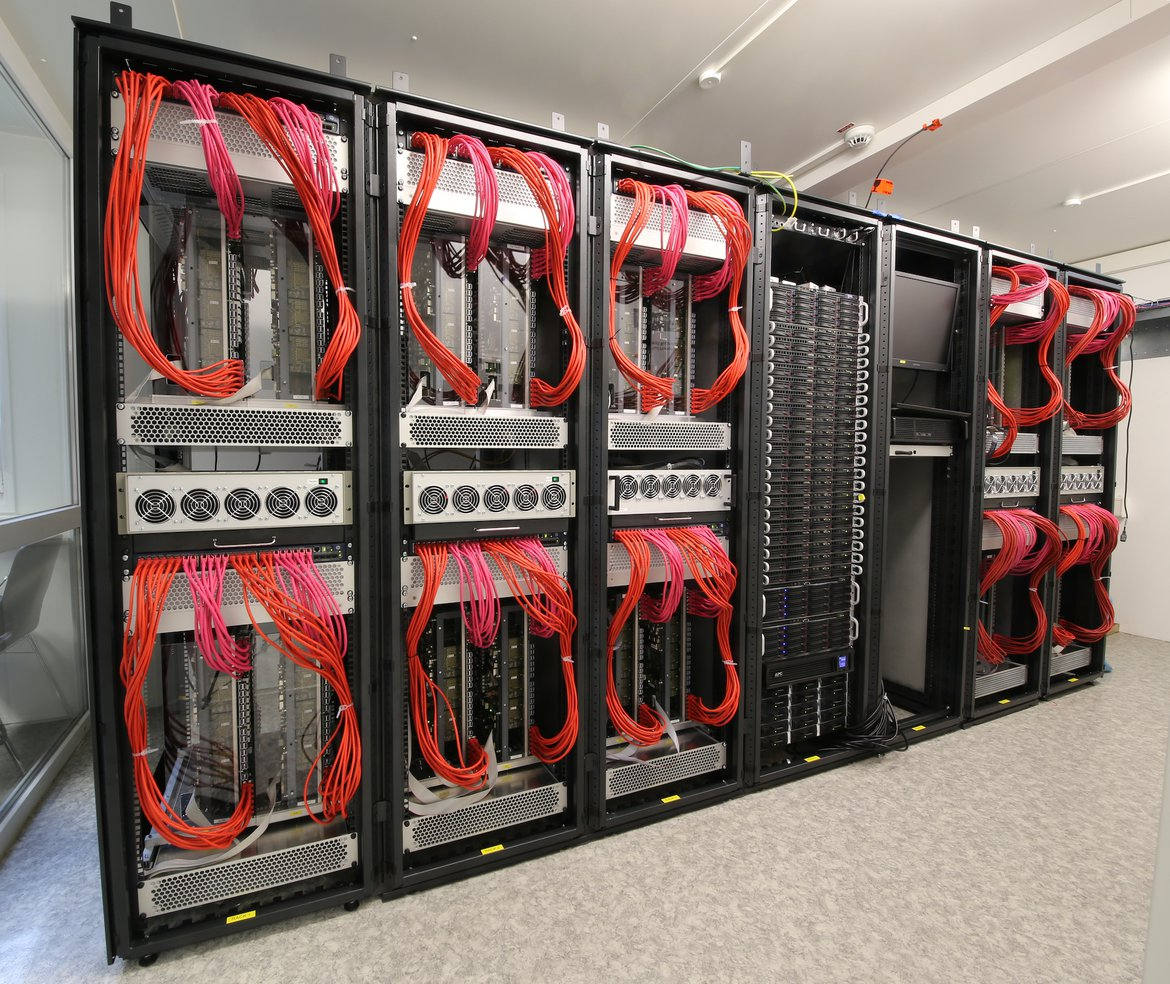
\includegraphics[width=\textwidth]{figures/brainscales.jpg}
        \caption{BrainScaleS supercomputer (image from \cite{nmp}).}
        \label{fig:brainscales}
    \end{subfigure}%
    ~ %add desired spacing between images, e. g. ~, \quad, \qquad etc.
      %(or a blank line to force the subfigure onto a new line)
    \begin{subfigure}[b]{0.53\textwidth}
        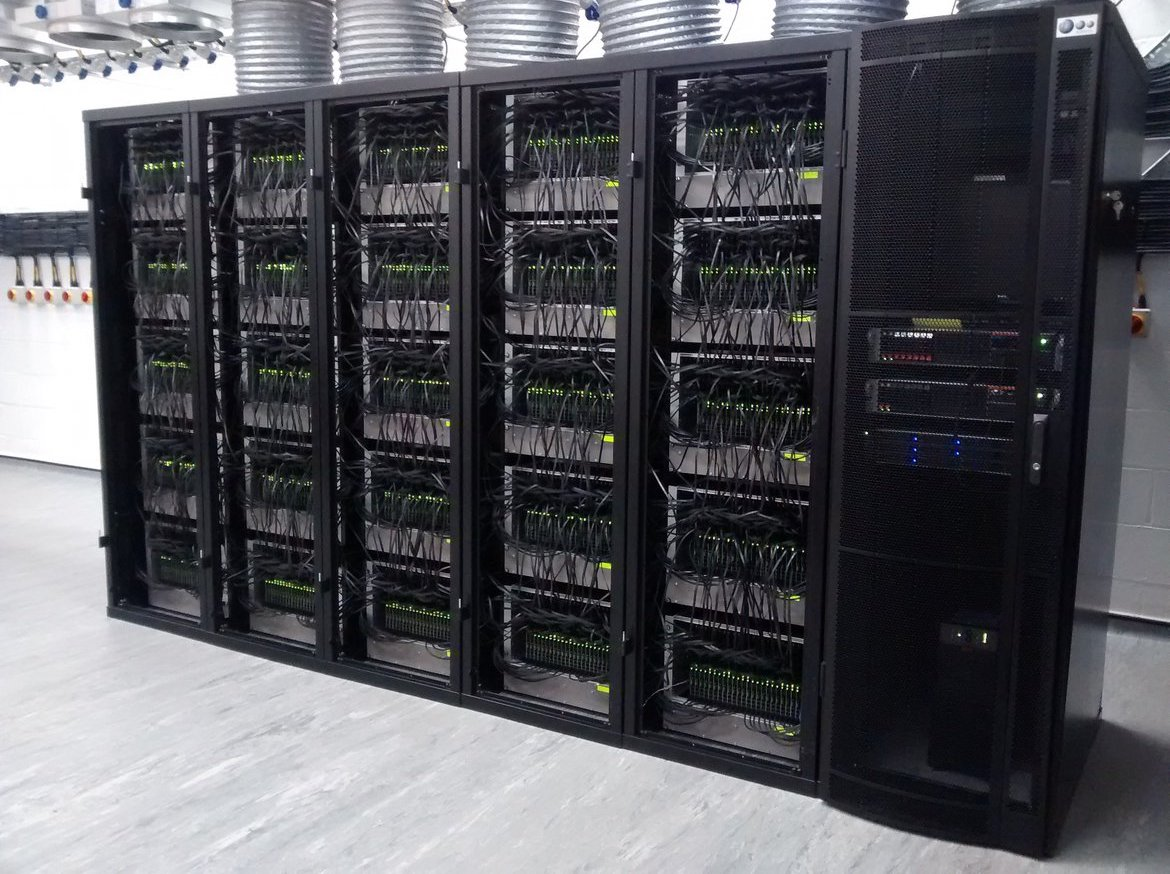
\includegraphics[width=\textwidth]{figures/spinnaker106.jpg}
        \caption{SpiNNaker supercomputer (image from \cite{nmp}).}
        \label{fig:spinnaker106}
    \end{subfigure}
%    \caption{Pictures of animals}
%    \label{fig:animals}
\end{figure} 

These two machines explore two different approaches to building a neuromorphic silicon brain. The BrainScaleS system is arguably the most neuromorphic approach, as it is based on the physical emulation of neurons using analogue and mixed-signals. Thus, there is no source code that the machine would execute step by step as in a von Neumann architecture computer. Rather, the system evolves according to the physical properties of the machine, running ten thousand times faster than a human brain would \cite{hw}. This means a day worth of real human brain training can be compacted in slightly over a minute, which drastically speeds up the workflow of neuroscientists experimenting with the machine. On a similar topic, it also seems noteworthy to mention Intel's Loihi \cite{loihi}, the state-of-the-art neuromorphic chip released in 2018, using an approach comparable to BrainScaleS, and that claims to outperform all existing hardware in its field. \\

Although this approach is faithful to the biology and is extremely energy efficient, it implements a fixed neuronal and synaptic model which restricts model exploration. This is why a second approach was taken with SpiNNaker, a neuromorphic computer of another kind where any neuronal and synaptic model could be implemented. As we use this machine for the project, we dedicate the next section to covering it in greater details. \\


%Over the years, distributed systems have become an evermore-essential tool for CPU-intensive applications. With the size of all the data available on the Internet currently doubling each two years, the processing power needs to follow a similar trend. For CPU-bound problems, scaling on distributed systems has been easier than for their IO-bound siblings. Inter-node communication in computer clusters is becoming the bottleneck for all these problems and the matter has received attention from the research community. From hot spot analysis in large scale shared memory multiprocessors \cite{hotspot}, to communication type \cite{perfcomp} and efficiency \cite {comm-eff} investigations, multiple attempts to optimise existing systems have been tried. \\
 
%However, another trend has emerged and tackles this issue in a radically different manner.

% Hot spot analysis in large scale shared memory multiprocessors
%-- [http://ieeexplore.ieee.org/document/1263548/]

% Performance bottlenecks on large-scale shared-memory multiprocessors
%-- [http://www-vlsi.stanford.edu/people/alum/pdf/0412_Kunz_FLASH.pdf]

% Performance Comparison of Message Passing and Shared Memory Programming with HPC Benchmarks
%-- [https://static.epcc.ed.ac.uk/dissertations/hpc-msc/2006-2007/0773421-27d-d07rep1.3.pdf]

% Distributed optimization for shared state systems: Applications to decentralized freeway control via subnetwork splitting
%-- [http://ieeexplore.ieee.org/document/7172081/]

% D-ADMM: A Communication-Efficient Distributed Algorithm for Separable Optimization
%-- [http://ieeexplore.ieee.org/document/6484993/]

% Asynchronous Distributed ADMM for Large-Scale Optimization—Part I: Algorithm and Convergence Analysis
%-- [http://ieeexplore.ieee.org/document/7423789/]



\subsubsection{SpiNNaker}

%With the Moore's Law historically exponential progress which is now slowing down and transistors that are reaching physical boundaries on how small they can be, other approaches have been attempted. In particular, brain-inspired computing \cite{bic} has received some attention over the past decades and some major initiatives in the field have been launched. The most significant one is the \euro{} 1B Flagship Human Brain Project of the EU, which aims to take the leadership of world research in neurmorphic simulations. Amongst the pillars of that project, it was essential to build a novel type of brain-inspired hardware that would be fit to run simulations of spiking neural networks. This is when the SpiNNaker project was born with a two-fold goal. Firstly, it should provide "a platform for high-performance massively parallel processing appropriate for the simulation of large-scale neural networks in real-time, as a research tool for neuroscientists, computer scientists and roboticists" \cite{SpiNNaker-Project}. Second, it should investigate how this brain-inspired novel architecture design could lead to new opportunities for massively-parallel computing. The hope is that areas other than neuroscience could benefit from the contribution SpiNNaker is making, which is precisely what we will be investigating.\\

Although the Human Brain Project \cite{hbp} was launched in 2013 with the EU funding, the SpiNNaker project had already started back in 2005. At the time, it was backed by the \textit{Engineering and Physical Sciences Research Council} (EPSRC), the main agency funding research initiatives in engineering and physics in the United Kingdom (UK). \\

\paragraph{Spin1 - test chip}

Working closely with neuroscientists, researchers from multiple UK universities spent years designing and experimenting to be able to deliver Spin1 in 2009, the SpiNNaker test chip Printed Circuit Board (PCB) \cite{dev-process}. It was intended as a proof of concept to demonstrate the design of the chip worked, and featured the first 4 SpiNNaker chips containing 2 ARM968 cores each. It was also formed of the common features that can be found on a PCB: power supply, LEDs, Ethernet interface as the primary communication channel with the host machine, SpiNNaker Link Connectors to chain multiple boards, extra testing facilities; see Fig.~\ref{fig:spin1} \\

\begin{figure}[!ht]
\centering
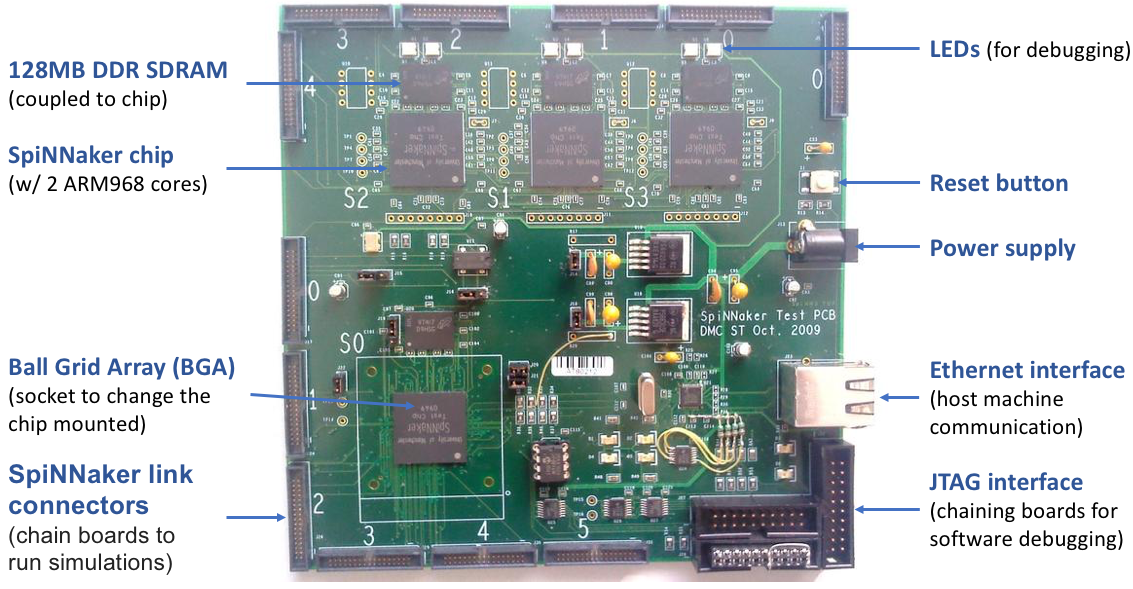
\includegraphics[width=\textwidth]{figures/spin1-schema.png}
\caption{Architectural schema of the Spin1 test chip PCB (image adapted from \cite{dev-process})}
\label{fig:spin1}
\end{figure} 


\paragraph{The challenge of power consumption}

Part of these testing facilities measured the energy consumption of the board. As a matter of fact, we know the human brain uses less than 20W to function so it was identified as a primary goal to build a PCB as energy-efficient as possible, even at the cost of some performance tradeoffs. Indeed, we are still far from properly understanding how the human brain works, but the knowledge we have of it has already taught us three lessons for building brain-inspired computers: massive parallelism, resilience to component failure and finally, energy-efficiency \citep{bic}. The latter was achieved at two complimentary layers:

\begin{itemize}
\item \textbf{Hardware}: the choice of the harware, and in particular of the ARM968 cores, was driven by energy efficiency. This is confirmed by the technical reference manual of the processor: \textit{the ARM968E-S processor is targeted at a wide range of embedded applications that require high performance, low system cost, small die size, and low power.} \cite{arm968} This class of processor takes low power usage as a compulsory requirement, and then tries to maximise the performance it can get out of the processor. Indeed, this core only runs at 200-MHz, which is an order of magnitude below the speed of a commodity PC processor. They typically power embeded devices, such as smartphones, and let the entire million-core machine run with at most 75 kW of electrical power during peaks \cite{spinnaker}. % Maybe say something about 1200*75 = 90kW !

\item \textbf{Software}: the programming model of the SpiNNaker Application Programming Interface (API) is event-driven. This paradigm allows the cores to be kept in a low-power state when they are not handling any events, which is not the case for the typical retail CPU. The ultimate goal of systems like SpiNNaker would be to achieve energy-proportional computing \cite{energy-prop}, where an idle core would not consume any power and where power usage would be proportional to the compute load of the core. As a mean of comparison, for a typical CPU in a data centre today, the power consumption is only divided by half when going from a full compute load core to an idle core, see Fig.~\ref{fig:energy-non-prop}. It would be interesting to see how far is SpiNNaker from being an energy-proportional computer, the benchmarks do not seem to have been published.
\end{itemize}
 
\begin{figure}[!ht]
\centering
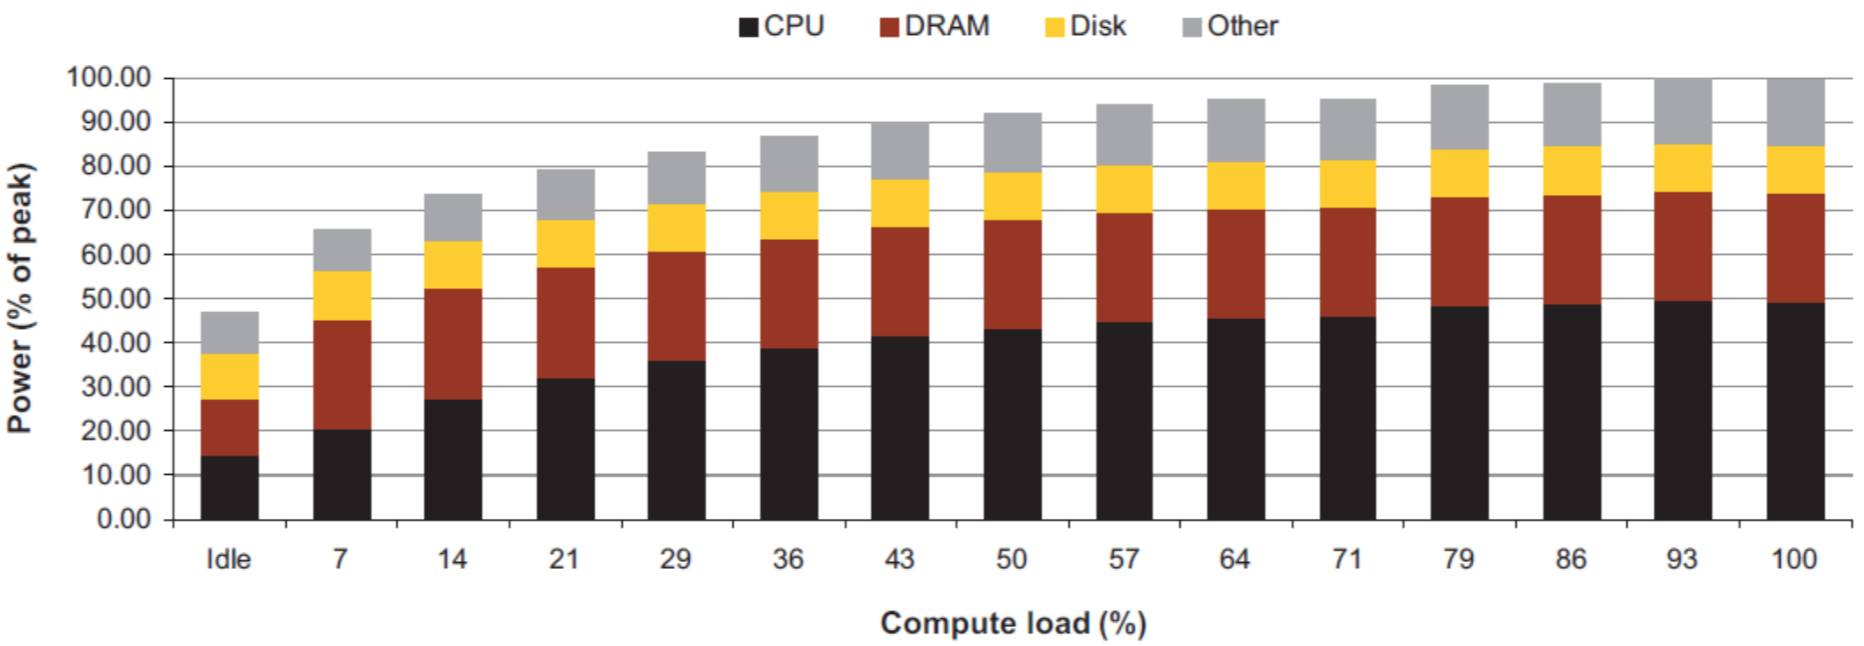
\includegraphics[width = 1\hsize]{figures/energy-non-prop.png}
\caption{Power consumption of a typical datacentre CPU (image from \cite{energy-non-prop}).}
\label{fig:energy-non-prop}
\end{figure}


\paragraph{Spin2 - production chip test}
 
After the success of the first Spin1 board, this new release from 2011 was mainly aimed at scaling \textit{up} the design. Each SpiNNaker chip would now embed 18 ARM968 cores instead of the 2 in the previous model. Moreover, the mobile Double Data Rate (DDR) Synchronous Dynamic Random-Acess Memory (SDRAM) was now embedded in the SpiNNaker chip package. Indeed, each chip has its own shared memory slot for all its cores to use. Additionally, a USB interface was added to allow the board to be reset remotely without having the press the physical button on the board. Finally, some of the extra elements used for testing in Spin1 (e.g. for power consumption) were removed as the board had already passed some of these tests; see Fig.~\ref{fig:spin2}.


\begin{figure}[!ht]
\centering
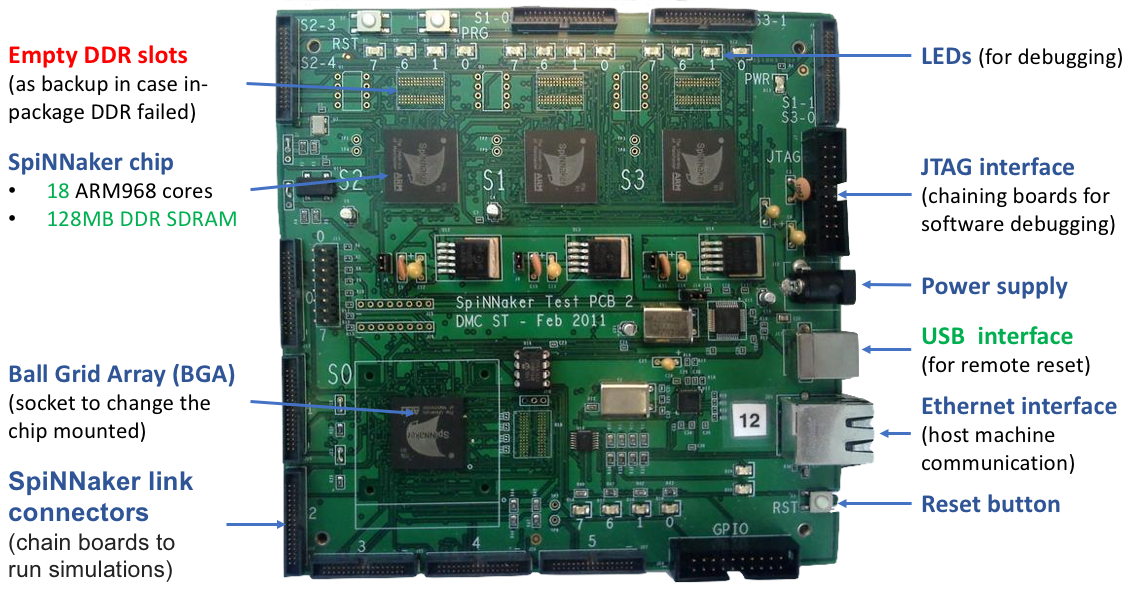
\includegraphics[width=\textwidth]{figures/spin2-schema.png}
\caption{Differential architectural schema of the Spin2 production chip test PCB, illustrating the design updated from Spin1 (image adapted from \cite{dev-process}).}
\label{fig:spin2}
\end{figure} 

\newpage
\vspace*{-1.2cm}
\paragraph{Spin3 - general purpose PCB}

Later in 2011, Spin3 was released after a few minor modifications to Spin2. The novelty of the board was to be general purpose, which made it the first usable SpiNNaker neuromorphic PCB for the research community. The surface of the board was also reduced by a factor of three, from $15 \times 15 = 225cm^2$ down to $8 \times 9 = 72cm^2$, to make it possible to fit it on a small robot. The design also got rid of all the hardware support for testing: BGA socket, power consumption monitoring, USB interface, reduced JTAG interface, reduced LED support per chip. Additionally, the number of SpiNNaker link connectors was also brought down to 2 as this board was not intended for large clusters of connected boards but rather for prototyping; see Fig.~\ref{fig:spin3}.

%\vspace*{-0.1cm}

\begin{figure}[!ht]
\centering
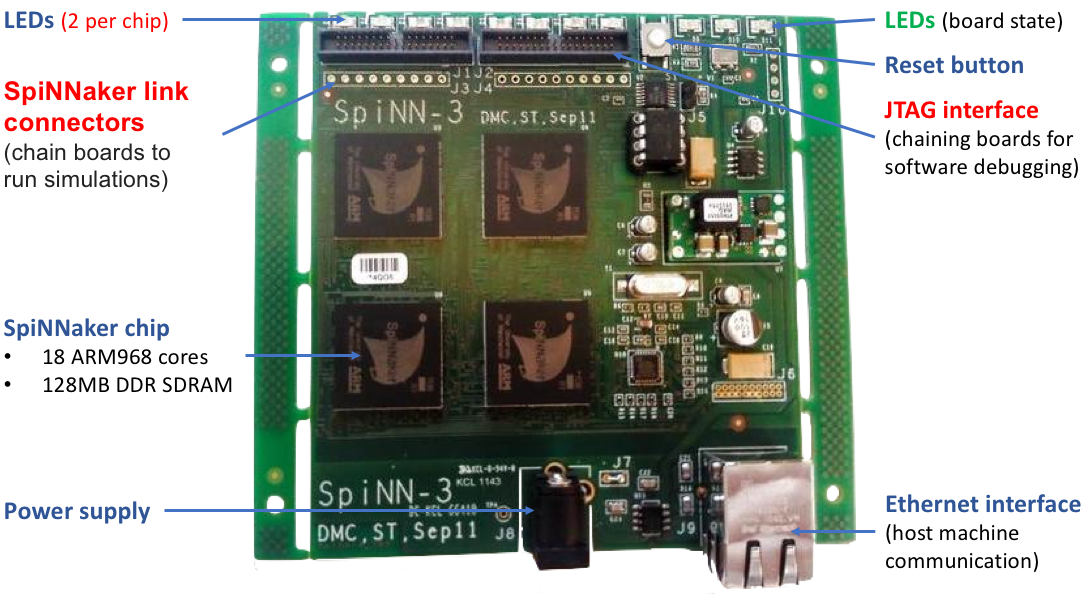
\includegraphics[width=\textwidth]{figures/spin3-schema.png}
\caption{Differential architectural schema of the Spin3 general purpose PCB, illustrating the design updated from Spin2 (image adapted from \cite{dev-process}).}
\label{fig:spin3}
\end{figure} 


\newpage
\paragraph{Spin4 - 48 chips PCB}

\begin{wrapfigure}{r}{0.4\textwidth}
  \begin{center}
    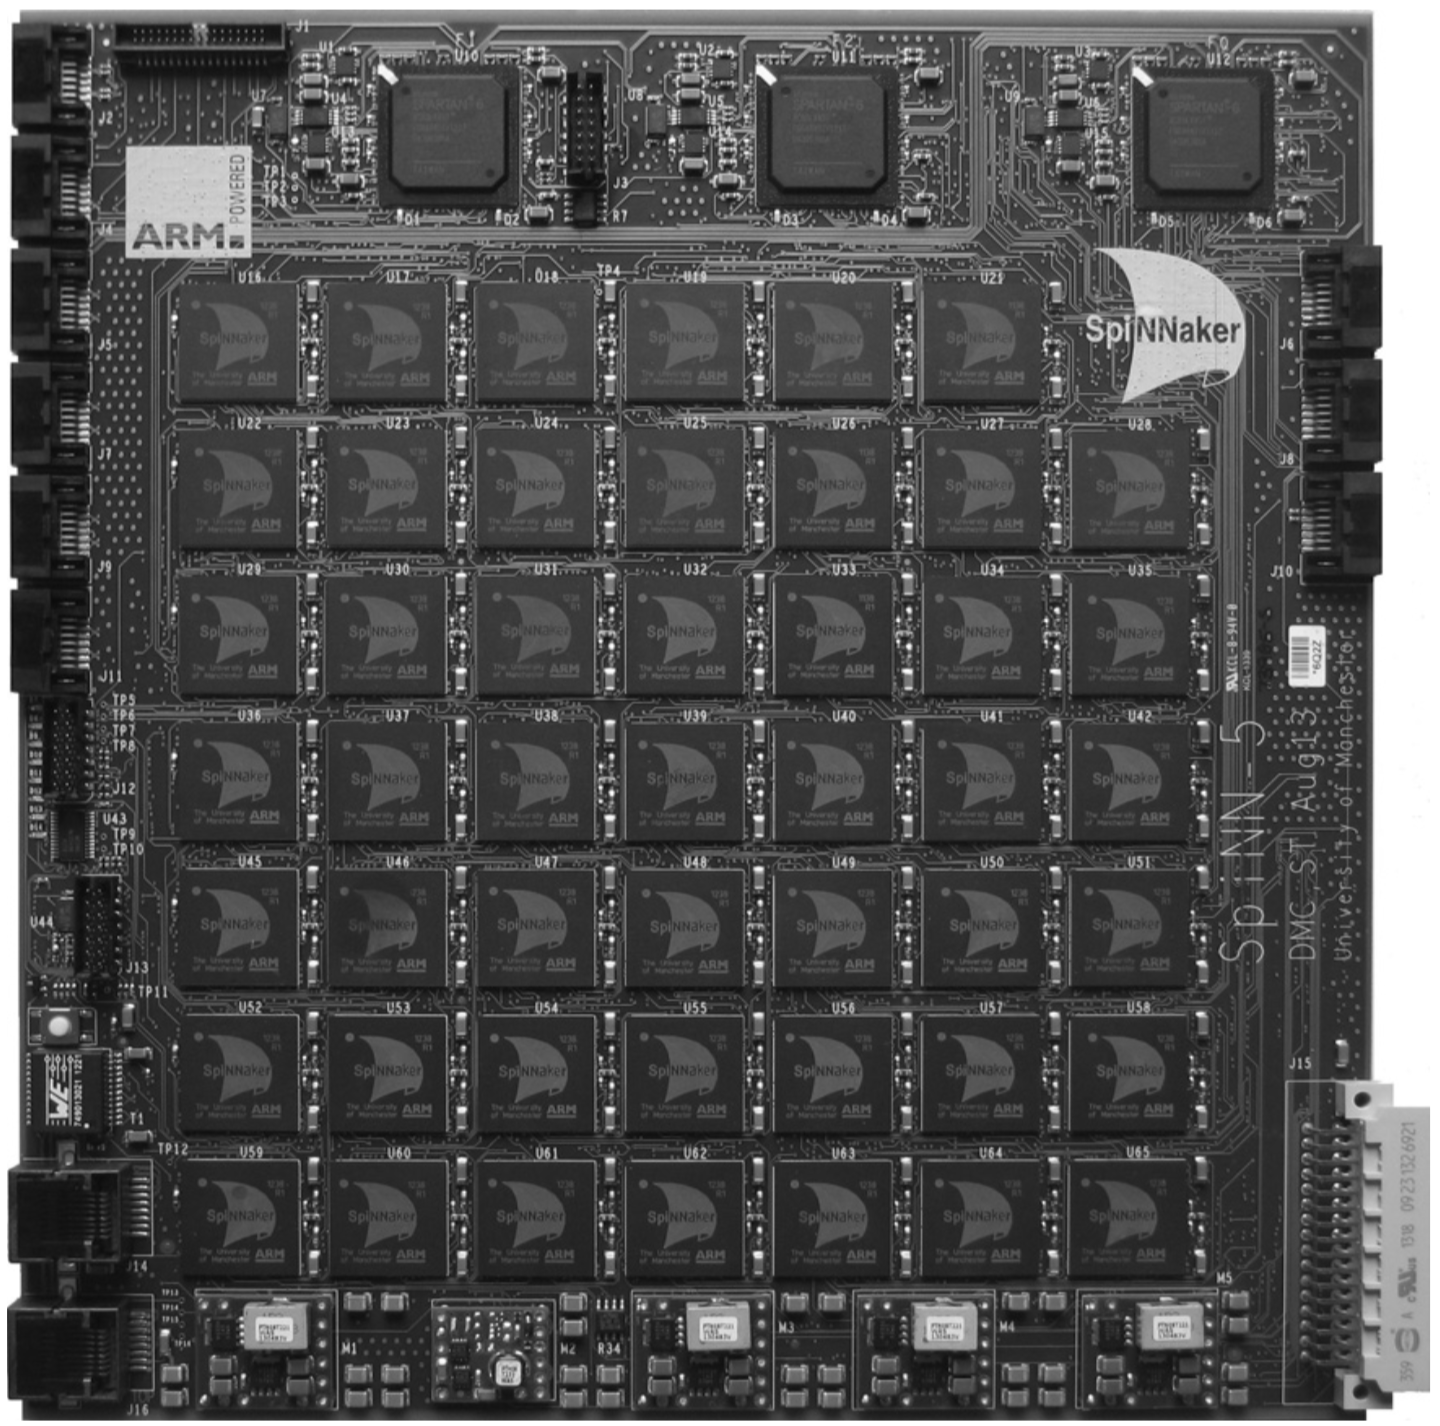
\includegraphics[width=0.38\textwidth]{figures/spin4.png}
  \end{center}
  \caption{The Spin4 PCB with 48 chips (image from \cite{bic}).}
  \label{fig:spin4}
\end{wrapfigure}

Finally, an ultimate version of the board was made to scale \textit{out} the previous design. At this stage, SpiNNaker chips had demonstrated they were functional so the main focus was to fit 48 chips on the same board. As a matter of fact, the ultimate goal of the project was to combine 1200 such boards and doing so would result in the million-core neuromorphic computer targeted. Indeed, $1200 \times 48 \textnormal{ chips } \times  18 \textnormal{ cores } \approx 1M \textnormal{ cores}$ and each core is expected to simulate a thousand neurons, which gives the expected one billion neurons real time simulation (and one million neurons per Spin4 PCB, see Fig.~\ref{fig:spin4}). As of today, the University of Manchester runs the largest version of the SpiNNaker machine with 500K cores, although they plan on expanding it over the coming months to reach the million of cores \cite{act-project-access}. \\ % TODO: don't we say they have a million somewhere? 
% Then, each SpiNNaker chip is mounted by group of 48 as an hexagonal array on a printed circuit board, which are then mounted as 24-board cages. The full SpiNNaker machine will be composed of 10 cabinets of 5 cages each, giving the expected $18\textnormal{cores} \times 48 \textnormal{chips} \times 24 \textnormal{board} \times 5 \times 10 = 1,036,800 $ processor cores.
 
Regarding power usage, the peak consumption of the Spin4 board was of 75W for a real time simulation of a million neurons \cite{dev-process}. As a comparison, IBM's TrueNorth chip, which has a design closer of BrainScaleS than SpiNNaker, is able to simulate one million neurons as well but only consumes 65mW of power while running a typical computer vision problem \cite{truenorthpaper}. But as BrainScaleS, TrueNorth has a physical model approach (see section \ref{sec:hbp}) so the power consumption comparison is probably unfair. Comparing SpiNNaker with the Sunway TaihuLight in China is probably fairer. It is now the second biggest supercomputer in the world (after newly released Summit stole the title on June 8th 2018 \cite{summit}) and number 20 on the GREEN500 list (top 500 supercomputers ranked by energy efficiency) \cite{green500}. The Sunway TaihuLight has 10,649,600 cores running at 1.45GHz for a power consumption of 15,371 kW \cite{top500} while SpiNNaker has 1,036,800 cores running at 0.2GHz for a power consumption of 75kW \cite{spinnaker}. By using an (approximative) performance per watt measure (usually in FLOPS/watts), we compute the ratio of the computer power (in GHz) over the power consumption (in kW), we find SpiNNaker more energy efficient by factor of 2.8:

\vspace*{-0.3cm}
\begin{equation*}
\begin{split}
R_{SpiNNaker} &= \frac{1,036,800 \times 0.2}{75} \\
R_{TaihuLight} &= \frac{10,649,600 \times 1.45}{15,371} \\
\frac{R_{SpiNNaker}}{R_{TaihuLight}} &\approx 2.8
\end{split}
\end{equation*}

However, computing the same ratio against the top GREEN500 computer, the Shoubu system B \cite{green500}, places SpiNNaker 7 times less energy efficient. Consequently, SpiNNaker probably does not defeat to current GREEN500 podium, but still achieves a very good energy efficiency that rivals with the state-of-the-art supercomputers in that matter. \\

Now that we have clearly described the hardware we will be using (the Spin3 board for the prototyping phase), let us now focus on how the internals of the machine actually work and interact.

% previous was "what we have", now is "how it works"
\subsection{SpiNNaker machine characteristics} \label{sec:smc}

First in section \ref{sec:hw}, we will focus on the hardware inside a SpiNNaker chip. Then, we will review in section \ref{sec:nw} the network topology that connects multiple chips together. Next, we will detail the transmission protocol used in that network - section \ref{sec:aa}. Finally in section \ref{sec:sw}, having it mind that physical layer, we will be able to understand what software stack was built on top of it to make the SpiNNaker machine a truly powerful tool.

\subsubsection{Chip architecture} \label{sec:hw}

The piece of hardware at the forefront of the design was the SpiNNaker chip (called a \textit{node} interchangeably), see Fig.~\ref{fig:spinn-core-labeled}. 

\begin{figure}[hbtp]
\centering
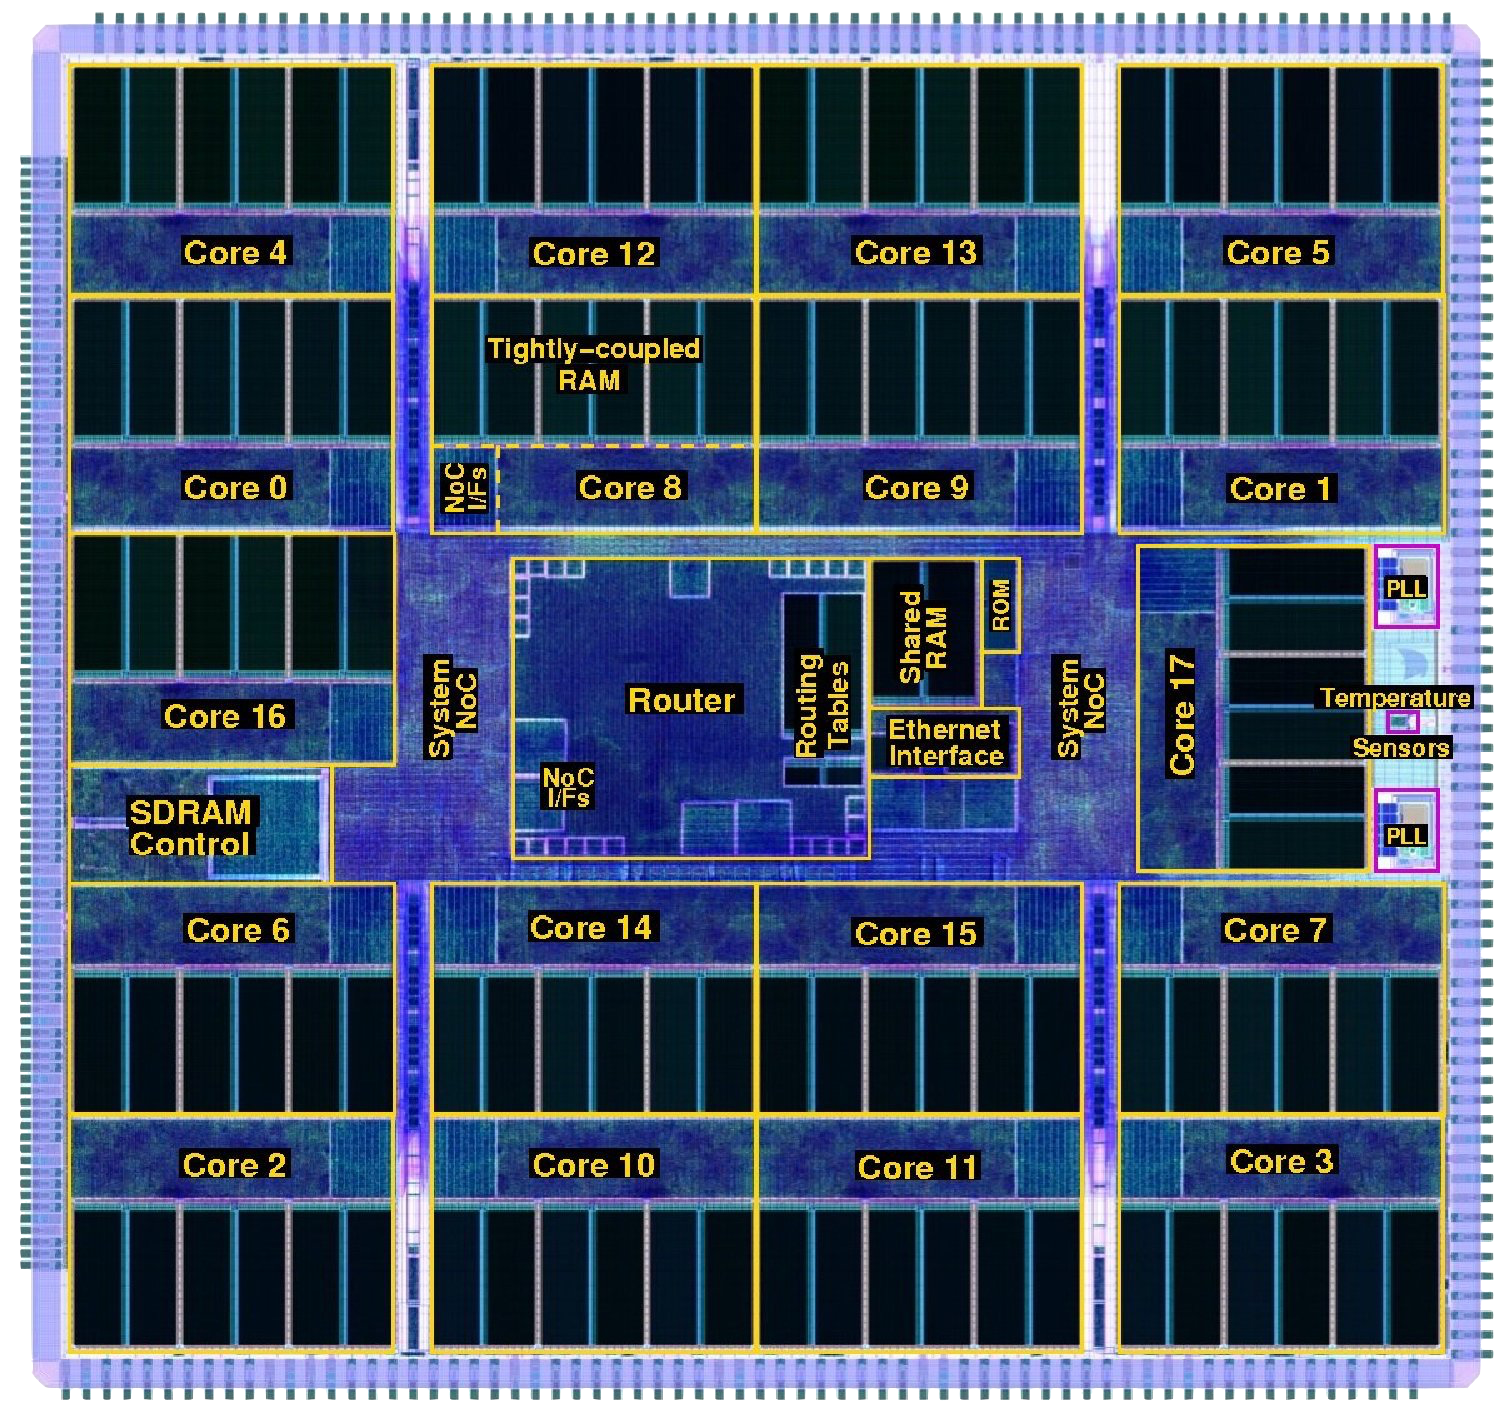
\includegraphics[width = 0.8\hsize]{figures/spinn_labeled_bw.png} 
\caption{The die plot of a SpiNNaker node, with 18 ARM cores (image from \cite{spinn-core}).}
\label{fig:spinn-core-labeled}
\end{figure}

Slides from a 2015 workshop \cite{spin-chip-resources} give an overview of the content of the chip:

\begin{itemize}
\item \textbf{Shared memory}: 128 MB of DDR SDRAM is shared between all the cores of the chip. It is located off-chip, but usually in the same package; hence the SDRAM controller as a on-chip interface to access it. In combination with 32 hardware locks on the chip, they allow powerful abstractions to be implemented, such as semaphores which we will use in the project implementation (detailed in section \ref{sec:prsf}).

\item \textbf{Router}: to forward packets in and out of the chip. Similar to the brain and as opposed to high-performance computers, SpiNNaker cores communicate via a packet-switched network optimised for large numbers of small fixed-sized data packets sent over UDP/IP (\textit{message passing}). Indeed on a regular computer, cores on the same chip usually share L2 or L3 caches and use it as a communication vector to synchronise computations reliably (\textit{shared memory}). To support multicast routing, where a packet sent once can be delivered to multiple destinations, a routing table of 256 associative entries \cite{testchip} can be configured to specify how to route each packet based on its key (detailed in section \ref{sec:nw}). Finally, we can note that using the User Datagram Protocol (UDP), a very simple transfer protocol with no fail-safe, is a deliberate biology-inspired design decision. UDP has no error checking, no packet sequencing and this built-in lack of reliability has led some people to refer to it as the 'Unreliable Datagram Protocol' \cite{udp}. Thus, it is fit to represent neuron-to-neuron interactions that are also based on a best-effort communication scheme.

\item \textbf{NoC}: Asynchronous Network on a Chip (NoC) that unifies the level of abstraction provided by the router, by allowing packets travelling between two cores of the same chip to be treated as any cross-chip communication.

\item \textbf{Cores}: 18 ARM968 cores running at 200MHz with a performance of 220 DMIPS. At boot time, each core will be assigned one role according to the following requirements: 16 application cores, 1 monitoring core and 1 spare core. The applications cores are the ones running the user code and implement a given simulation, such as a spiking neural network. The monitoring core is responsible for coordinating the work of the application cores. For instance, any command that comes from the host machine is targeted to the monitoring core, that will then execute that command on the application cores it manages. Lastly, a spare core is a redundancy added for defect-tolerance, taking here again some inspiration from the brain which looses about 200,000 neurons a day unnoticed \cite{neuron-loss}. 

To equip each core, they all come with a DMA controller, to copy from and to shared memory at a low latency (15ns)\cite{spin-chip-resources} and without a CPU overhead. Additionally, each core comes with a communications controller (to interface with the router) and a vectored interrupt controller (to support the event-driven programming paradigm of SpiNNaker).

\item \textbf{TCM}: Each core also has 96KB of Tightly Coupled random-access Memory (TCM), that is mounted on top of the core to minimise latency (5ns) \cite{spin-chip-resources}. This memory space is partitioned into two dedicated memory subspaces: 32KB of Instruction TCM (ITCM) where the active binary is loaded and 64KB of Data TCM (DTCM) to be freely used by the program running on the core.
\end{itemize}

The following hardware elements are part of the chip internals tools, and are mainly used by the monitor processor (used interchangeably with \textit{core}):

\begin{itemize}
\item \textbf{Ethernet} interface: used for interactions with the host machine. The monitor core is in charge of handling these interactions.

\item \textbf{System ROM}: a 32KB memory space with that is executed on chip start up to boot the system. It first runs a self-test, then starts the monitor processor selection process, bootstraps the router and eventually boots the remaining components of the chip \cite{testchip}.

\item \textbf{System RAM}: a 32KB memory space used primarily by the monitor core to optimise its system operations.

\item \textbf{Sensors}: three sensors to record temperature variations on the chip; remainders from the testing stages of the chip.

\end{itemize}

When the chip starts, the self-test phase of the System ROM will identify all valid cores. For example, if a core is detected to have failed, the algorithm will decide to use the spare core but that will remain invisible to the end user. Indeed, SpiNNaker defines a notion of Virtual Core \cite{vcpu} where each running core has both a physical identifier (hardware core ID) and a virtual identifier (exposed to user). Once the monitor processor selection has ran and chosen a core at random, it returns the physical identifier of this core which is mapped to the Virtual Core 0. Then, up to 16 physical cores are assigned a virtual identifier following an incrementing counter. These virtual identifiers help make the chip resilient to core failures, without exposing any of the hard-coded identifiers that might fail, always returning a list of consecutive and functional cores. This design is similar to hard disk drives, which have a physical mapping of sectors but will only expose a logical mapping of these sectors that factors out bad sectors. \\

After this overview of how a chip works, let us see how multiple chips work together and how data flows through SpiNNaker. 

\subsubsection{Network topology} \label{sec:nw}

The SpiNNaker chips are arranged in a 2D triangular mesh network with bidirectional links to 6 neighbours \cite{testchip}, as show on chip (1,1) in Fig.~\ref{fig:mesh}.

\begin{figure}[hbtp]
\centering
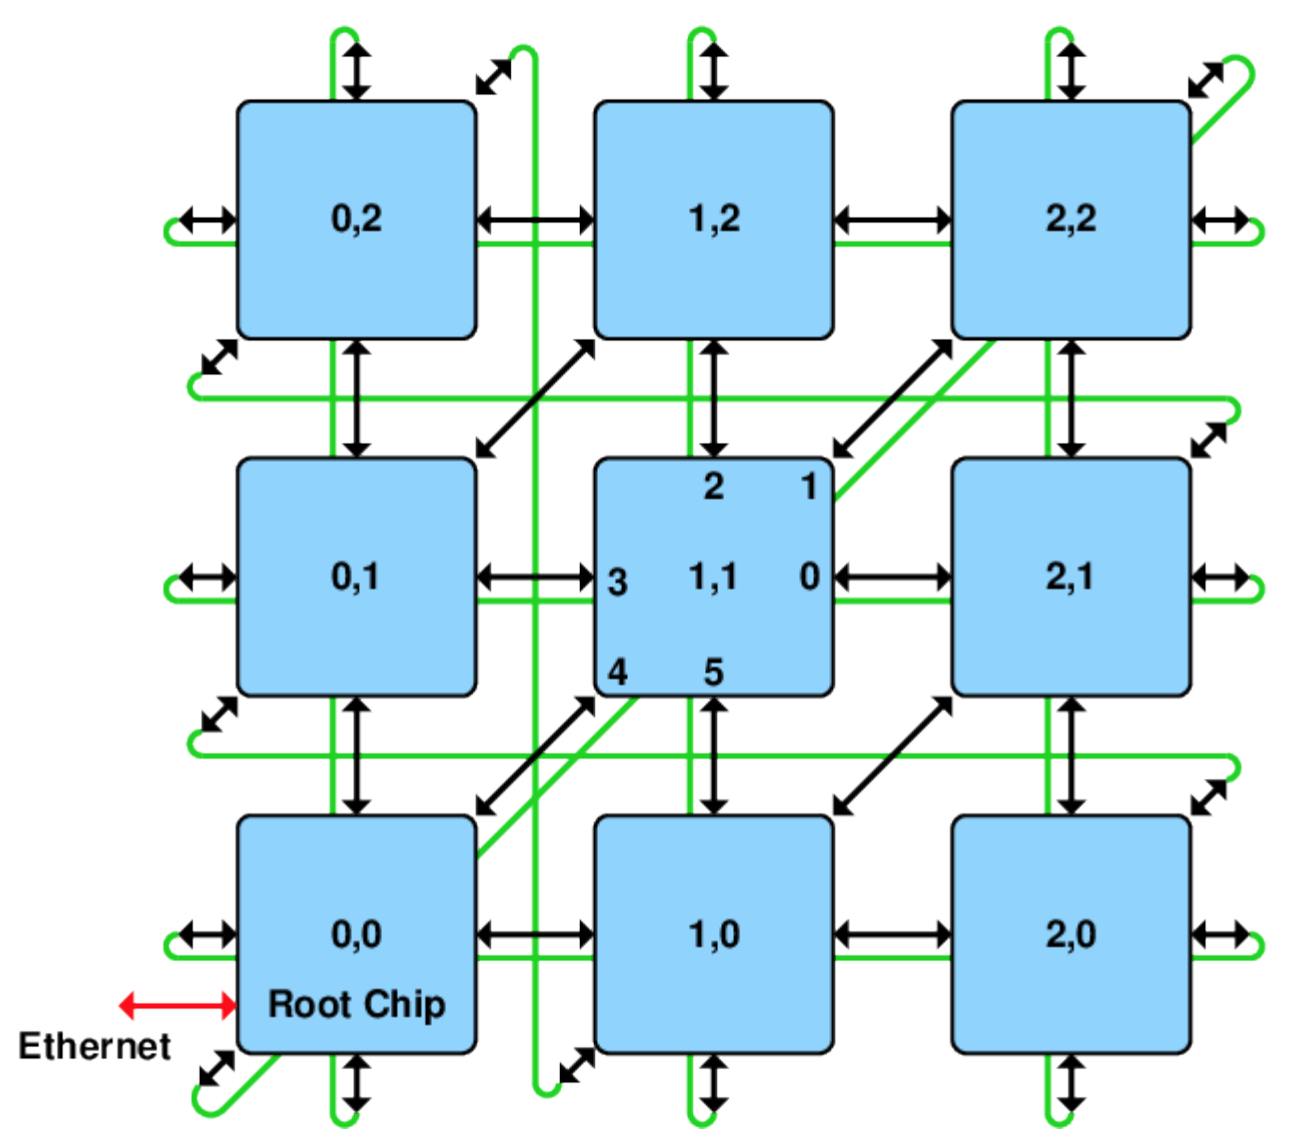
\includegraphics[width = 0.8\hsize]{figures/mesh.png}
\caption{2D mesh network interconnecting SpiNNaker chips (image from \cite{mesh_img}).}
\label{fig:mesh}
\end{figure}

During system bootstrap, a flood-fill discovery mechanism identifies all the chips available and initialises a 2D array of SpiNNaker chips that is exposed to the host machine. The similarity with Virtual Cores is clear, and this logical mapping has the advantage of allowing for dynamically changing network topologies at boot time. The host machine, connected to one of the circuit boards by a 100Mbit/s Ethernet cable, designates the root chip: the chip (0,0) on that connected board. Then, at boot time, the chip will discover the chips around it on the same board, which will in turn discover all the connected boards with their chips. Another advantage of this dynamic topology is defect-tolerance, where a defective chip can simply be removed from the network logical mapping. \\

Now that the network structure is clear, let us see what data flows through it by giving an overview of the transmission protocols used to move data in SpiNNaker. \\


\subsubsection{Data transmission protocols} \label{sec:tp}

\paragraph{Packet format}  \label{sec:pf}

Each core has its own communications controller that is responsible for formatting outbound packets and parsing those incoming. Any SpiNNaker packet will be of either 40bits or 72bits (with a 32bits payload) and will be of one of the following four forms \cite{testchip}:

\begin{itemize}
\item \textbf{Multicast (MC)} packet, sent once and potentially has multiple destinations. Routing is determined by a key given by the sender. 

\textit{Usage}: primary communication format for application cores that propagate neural events to other application cores in the system.

\item \textbf{Point-to-point (P2P)} packet, unicast transmission between a source and a destination core. 

\textit{Usage}: system management, e.g. to load a given executable on a core.

\item \textbf{Nearest-neighbour (NN)} packet, unicast or broadcast transmission with  neighbours. The neighbours are the six directly connected chips, as show on Fig.~\ref{fig:mesh}. For a unicast transmission, the target will be one of these neighbours or the local monitor processor on the chip. For a multicast transmission, the packet will be sent to all six neighbours.

\textit{Usage}: system flood-fill algorithms, e.g. for discovery when bootstrapping the system.

\item \textbf{Fixed-route (FR)} packet, unicast transmission with the host system.

\textit{Usage}: to move debugging data from a core back to the host machine.

\end{itemize}


\paragraph{SpiNNaker Datagram Protocol (SDP)}

For the sake of completeness, we also need to mention the SpiNNaker Datagram Protocol (SDP) \cite{sdp}. This protocol operates at a higher level that the packet formats above, and combines multiple point-to-point packets (which define a notion of packet sequencing) to move blocks of up to 256 bytes of data in a SpiNNaker system. As all communications in SpiNNaker are based on a best-effort principle, the delivery of any message sent cannot be guaranteed. Additionally, these packets can travel out of SpiNNaker to the host machine through the Ethernet link between the two. In that case, the full SDP packet is wrapped as the payload of a UDP packet. \\

Let us take the typical example of the host machine commanding a Spin3 board to switch on the LED of chip (1,1). The host machine software (thoroughly reviewed in section \ref{sec:sw}) will create an SDP packet targeted at chip (1,1), and will wrap it in UDP packet to send it over UDP/IP to the board. The root chip (0,0) will be the one receiving the packet, and its monitor processor will be the one accepting the communication. It will unwrap the SDP packet and forward it to chip (1,1) using point-to-point routing. If the SDP packet is too big, multiple point-to-point packets will be used with a sequencing mechanism for ordering. When arriving in chip (1,1), the monitoring processor of that chip will handle the reception of the packet. Its communication controller will then decode the instruction sent by the host machine telling it to switch its LED on. Then, that is it, no confirmation is sent back to the host machine: SpiNNaker is a best-effort world.


\paragraph{Multicast routing data packet}

Any developer for SpiNNaker will mostly be interested in Multicast (MC) routing to exchange data between the application cores where the binaries of its simulation lives. The exact structure of an MC packet is showed in Fig.~\ref{fig:mc_pkt_layout}:

\begin{figure}[hbtp]
\centering
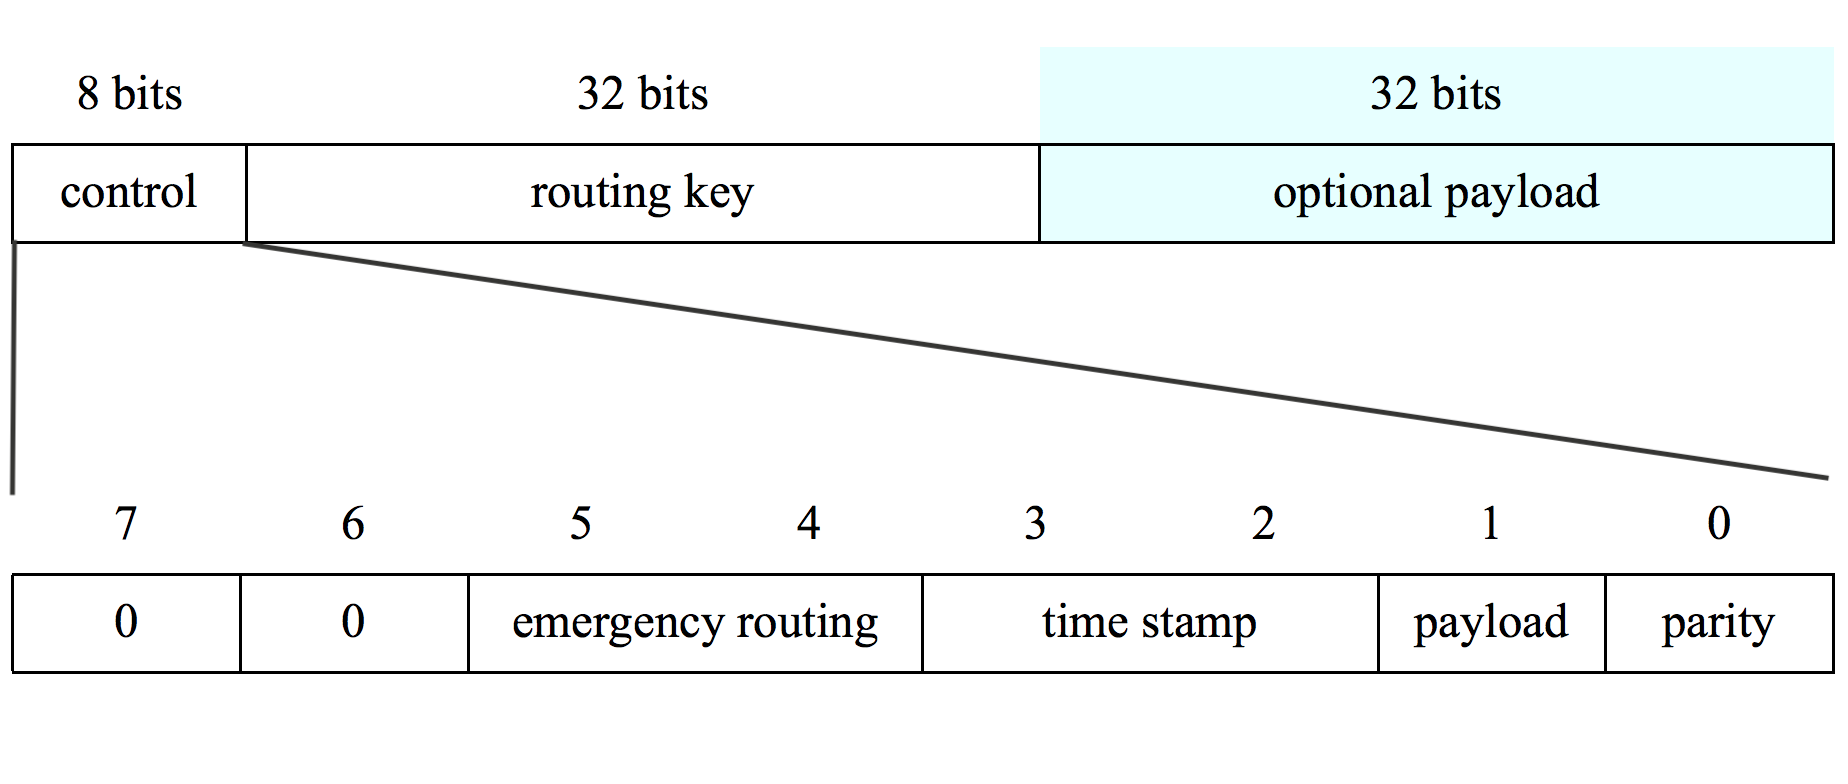
\includegraphics[width = 0.95\hsize]{figures/mc_pkt_layout.png}
\caption{Structure of a Multicast packet in SpiNNaker (image adapted from \cite{mc_pkt_layout}).}
\label{fig:mc_pkt_layout}
\end{figure}

As mentioned earlier, it is a 72-bit data frame where the routing key and the payload take up 32 bits each. Additionally, there are eight more bits of metadata that are used for management. The first two bits define the type of packet sent: \texttt{00} for MC, \texttt{01} for P2P, \texttt{10} for NN, \texttt{11} for FR. Then, the next two bits for emergency routing are stateful and can change depending on routing conditions. If a link fails or becomes congested at run time, this additional information will be updated and will help the local router find alternative routes. Then, the next two bits encode a global cycling four-step time stamp that is set by the packet sender. It allows late packets to be detected and dropped to ensure no \textit{errant packet} stays indefinitely in the network. Then, the payload bit signals if the packet has a payload or not. Finally, a parity bit is used to check for transmission errors. \\

% This design mimics how neurons fire action potentials, also called "spike" for the sake of simplicity. Each of these data packets is 40 bits long, the first 32 b being the source neuron AER identifier while the last 8 b are used for management. AER is the Address Event Representation which is a widely accepted encoding to describe neural activity and how information is exchanged between neuromorphic hardware-based neurons \cite{aer}. This design lets a single SpiNNaker core process up to 5 million connections/s. \cite{spinnaker} \\

Now that the physical components of SpiNNaker have been described, let us focus on the dense software stack that make this powerful tool usable.

\subsubsection{Software architecture} \label{sec:sw}

The software stack involved in a SpiNNaker simulation is summarised in Fig.~\ref{fig:software_stack}:

\begin{figure}[hbtp]
\centering
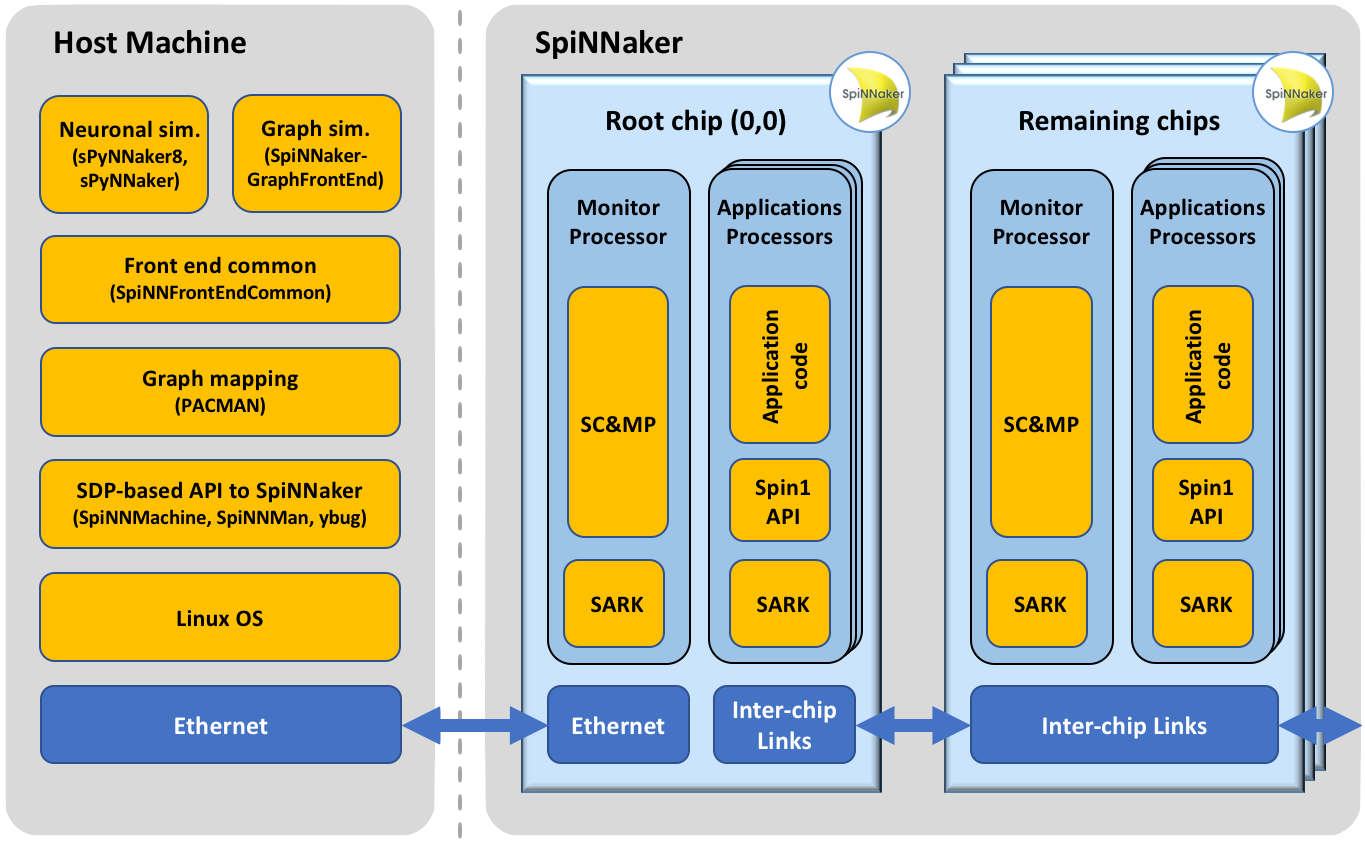
\includegraphics[width = 1\hsize]{figures/software_stack.png}
\caption{Structural diagram of the SpiNNaker software stack (image adapted from \cite{spinnaker}).}
\label{fig:software_stack}
\end{figure}

We will now detail thoroughly each module and its role within the entire stack. All these modules can be classified in one of the following three categories:

\begin{itemize}
\item \textbf{Host Machine}: this is the machine that the user is logged on, and where all the higher-level software resides. For example at the highest level, a spiking neural network simulation would be described in \texttt{sPyNNaker}, at a lower level neurons would be mapped to a SpiNNaker core in \texttt{PACMAN}, and even lower the compiled C application binaries sent to SpiNNaker through \texttt{SpiNNMachine}.

\item \textbf{Monitoring Processor}: runs the SpiNNaker Control and Monitor Program (SC\&MP) \cite{spinnaker} that contains all the monitoring-specific logic. At the foundation of any SpiNNaker core we also find the SpiNNaker Application Runtime Kernel (SARK) \cite{sark}. It is the lowest layer of software that provides functionalities such as core and application bootstrapping, memory management, interrupt control, handling of host machine commands on the monitor processor (e.g. remote memory alteration for debugging, application load / unload).

\item \textbf{Application Processor}: runs the simulation binary compiled from C on the host machine by the user. Two libraries providing support to the application code can also be statically linked with the binary. The first one is SARK, which is compulsory as it supports the application cores in the SpiNNaker environment. The second one is spin1, an event-based API that operates at a higher level and lets the user define callbacks for specific events.
\end{itemize}

All of these software tools will be detailed in turn in the following sections. The software running on the host machine is written in Python and binaries ran on SpiNNaker are first compiled from C on that machine as well. Then, the binaries are sent to the board for execution. \textit{Note}: in the following sections, we use the formatting convention \texttt{$\ll$Repository$\gg$} to name a software module that can be found on GitHub at \href{https://github.com/SpiNNakerManchester}{https://github.com/SpiNNakerManchester/$\ll$Repository$\gg$}.

\paragraph{Host Machine software}

The software stack running on the host machine is by far the most complex, because many distinct modules execute a specific task which is not always easy to grasp for the newcomer. Moreover, the user is likely to only directly touch the top layer of the stack which hardens a global comprehension of these modules. We will follow a top down approach to cover them all. \\

At the very top of the stack, there are two frameworks that can be used to define a simulation: \texttt{sPyNNaker8} for spiking neural networks and \texttt{SpiNNakerGraphFrontEnd} for generic graphs. The former, \texttt{sPyNNaker8}, is an implementation of PyNN, a \textit{simulator-independent language for building neuronal network models} \cite{pynn}. The software stack is actually further divided into \texttt{sPyNNaker}, a version-independent port of PyNN on SpiNNaker, and \texttt{sPyNNaker8}, a version-specific interface to sPyNNaker implementing PyNN version 0.8. This framework is specific enough that it can derive all the C application code from the high-level description of the simulation in Python. On the other hand, \texttt{SpiNNakerGraphFrontEnd} is a more generic framework and requires the user to define both Python graph specification and application code to be run on SpiNNaker. It makes it more flexible, but also makes the start-up cost of any serious project much higher as much of the logic needs to be handcrafted (e.g. routing). \\

A level below, there is \texttt{SpiNNFrontEndCommon} which holds all the common tools that are used by both front-end frameworks. For instance, it defines many 
Python abstract classes that define very specialised behaviours and that are combined together in the frameworks to create custom SpiNNaker elements. For instance, a Python class for a vertex in the \texttt{SpiNNakerGraphFrontEnd} could derive from the abstract class \href{https://github.com/SpiNNakerManchester/SpiNNFrontEndCommon/blob/master/spinn_front_end_common/abstract_models/abstract_has_associated_binary.py}{\textit{AbstractHasAssociatedBinary}} to indicate the class has an associated C code binary file. \\ % TODO: take a real example from a framework

Another level lower, this is the graph mapping algorithm called \texttt{PACMAN}. It takes as input the graph representing the simulation, whether it is a list of custom vertices or of interconnected neurons, and maps them to virtual SpiNNaker cores while complying with a given list of constraints. For instance, let us take the example of a graph of custom vertices that take up a lot of TCM such that a small number of vertices could fit on a SpiNNaker core without exhausting its resources. We would be able to call \texttt{PACMAN} with this graph and a list of constraints detailing the resource requirements of a single vertex, and \texttt{PACMAN} would figure out, say, only 100 of these vertices could fit on a single core and would return a mapping from the input graph to the virtual cores of the SpiNNaker machine. \\ 

Going another layer below, there is the ultimate collection of software modules that directly interact with SpiNNaker using SDP over UDP/IP. For a simulation triggered from one of the front-end frameworks, \texttt{SpiNNMan} will be used alongside one of its dependencies: \texttt{SpiNNMachine}. \texttt{SpiNNMan} is an interface to the SpiNNaker boards that is used by the higher layers to communicate with the machine. Consequently, it contains a set of functions that can be used to send messages to the board, spin up application cores, load binaries, and more. \texttt{SpiNNMachine} however is simpler and only provides a hierarchy of Python classes to represent the SpiNNaker machine. Finally, an interesting Command Line Interface (CLI) is \textit{ybug}, which can be found in the tool-kit repository \texttt{spinnaker\_tools}, and allows the user to directly interact with the machine. It is a Perl script that provides functionalities similar to \texttt{SpiNNMan} (e.g. cores boot, application loading, retrieving logs), but it runs as an interactive shell which empowers the developer with a practical solution for live inspection of the system. \\

As mentioned above, the SpiNNaker tools in \texttt{spinnaker\_tools} form another important module. It features the source code of important SpiNNaker binaries, such as SC\&MP, SARK and spin1, but also contains Perl scripts for tooling, such as ybug and some more visualisation GUIs not used by that project. \\

All in all, the software stack of the host machine piles up relatively high, and a good overview of the role of each module is a significant edge towards becoming a proficient SpiNNaker developer. Now let us focus on the binaries that run on SpiNNaker (after being compiled and transferred from the host machine).


\paragraph{Monitoring Processor software}

\begin{figure}[hbtp]
\centering
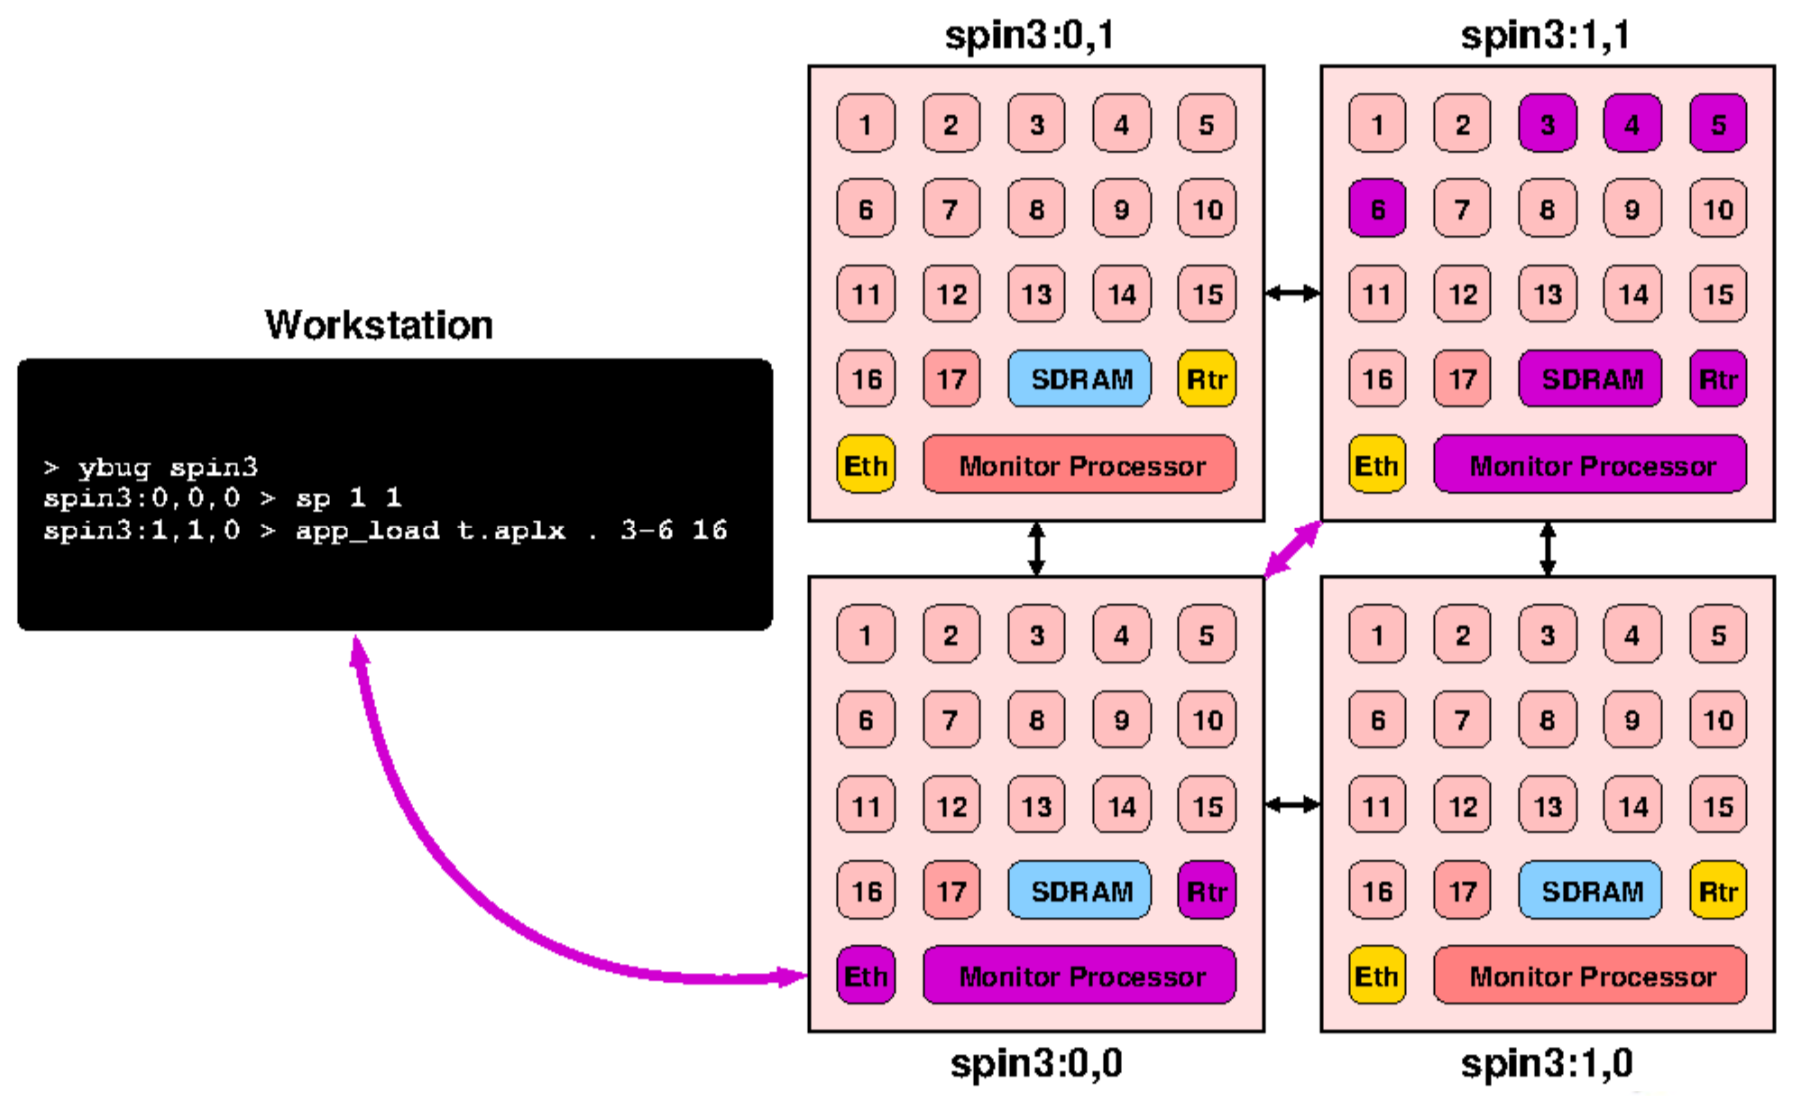
\includegraphics[width = 1\hsize]{figures/ybug.png}
\caption{Application loading using \textit{ybug} (image from \cite{ybug}).} % Check image ref
\label{fig:ybug}
\end{figure}

Focusing now on the Monitoring Processor, the main software component is the SpiNNaker Control and Monitor Program (SC\&MP). The program is loaded on all the monitoring cores during the system bootstrapping phase and oversees the operations of an entire chip. It handles any command received from the host machine using the SpiNNaker Command Protocol (SCP) \cite{ws6} (transmitted over SDP), and executes them. For the monitoring processor on the \textit{root} chip (on board directly connected to the host machine), SC\&MP will also inject in the SpiNNaker network any inbound packet received from the host. For instance, if a developer uses \textit{ybug} to load application \textit{t.aplx} on cores 3 to 6 of chip (1,1) with the application ID 16, the generated SDP packets would cross the hardware elements shown in Fig.~\ref{fig:ybug}. \\

Another important piece of software is the SpiNNaker Application Runtime Kernel (SARK) \cite{sark} library. It is required on all SpiNNaker cores and implements the following three functionalities:

\begin{itemize}
\item \textbf{Bootstrapping}: initialises all cores, memory stacks and control registers. Then, it calls the application \textit{c\_main} function which acts as the \textit{main} of a C program: it is the entry point of the application code that starts the simulation.

\item \textbf{Utility tooling}: for low-level interaction with the chip, e.g. memory management, interrupt controller, LEDs state update. It also implements some higher-level constructs, such as per-core 8-bit semaphores that are implemented using a combination of DTCM and hardware locks.

\item \textbf{Extra tooling for monitoring processor}: mainly to handle host machine commands using SCP/SDP (SpiNNaker Command Protocol over the SpiNNaker Datagram Protocol). This is the code that will handle any ybug-issued command targeted at the chip it is on.
\end{itemize}

Finally, let us see the application cores which run the code written by the developer.

\paragraph{Application Processor software}

On all application cores, SARK will need to be loaded as well as it provides the basic and compulsory framework for any application binary. Additionally, an optional library can be linked with the application binary and provides support for an event-based API. In SpiNNaker's manycore paradigm using message passing, it is likely the developer will want most (if not all) of the logic of its simulation to run as an event handler. For example in a spiking neural network, the application code will want to handle incoming spikes arriving and potentially propagate a new spike as a response to that event. To help the developer in doing so, the SpiNNaker Application Programming Interface (API), abbreviated \textit{spin1}, was built. It allows the user not to worry about the control flow of its simulation and only focus on the data flow by defining callbacks. Four types of events can be handled \cite{spinnaker}: 

\begin{itemize}
\item \textbf{Incoming packet}: handle a packet that just arrived. A different callback can be registered for each of the four types of packet that can be received (see section \ref{sec:pf}).

\item \textbf{DMA complete}: when the DMA controller finished an operation.

\item \textbf{Timer tick}: to implement time awareness, the core 'ticks' every millisecond (configurable) to increment its local notion of time.

\item \textbf{User event triggered}: it is a software-triggered interrupt to let the user handle a custom event.
\end{itemize}

Each of these callbacks can be dynamically registered and unregistered at runtime using \textit{spin1}. Moreover, a priority needs to be given to each of these callbacks at registration to define which callback should run first when two events occur at the same time. As in Unix niceness for processes, the lower the value of that priority, the higher the priority. Two different types of priorities can be registered:

\begin{itemize}
\item \textbf{Queueable callbacks}: their priority value is $\ge 0$. If a callback with a lower priority value is already running, they will be queued by the scheduler. However, they will pre-empt any running callback with a higher priority value.

\item \textbf{Non-queueable callbacks}: their priority is $-1$. They execute immediately without possibility of being interrupted, pre-empting any running callback. For this properties to hold at any time, only a single non-queueable can be defined per core. Otherwise, if two such callbacks were defined and triggered at the same time, one would end up pre-empting the other or one would not be executed immediately.
\end{itemize}

Overall, these libraries equip the developer with a comprehensive set of tools that let simulations be defined at different granularities. Now that we have described the set of tools available to us, developers who want to port Page Rank to SpiNNaker, let us review how SpiNNaker can actually be used. \\

\subsection{SpiNNaker usage} \label{sec:usage}

As explained, SpiNNaker (Spiking Neural Network Architecture) was built for spiking neural networks simulations. This is the reason why a lot of effort was put into having the \texttt{sPyNNaker} / \texttt{sPyNNaker8} front-end frameworks expose a very high-level API entirely in Python. It makes the tool very user-friendly and enables researchers to quickly craft a simulation without bothering with its implementation technicalities. We will first be discussing spiking neural network simulations in section \ref{sec:snn}, and will then focus on alternatives applications of SpiNNaker together with their implementation in section \ref{sec:aa}. All the use cases described will be relevant because the design decisions of the Page Rank implementation in this project depends on an understanding of the benefits and drawbacks of each example's approach.

\newpage % TODO: remove me
\subsubsection{Spiking neural networks} \label{sec:snn}

First, let us go through a brief biology refresher to properly define what a neuron, an axon and a synapse are.

\begin{figure}[hbtp]
\centering
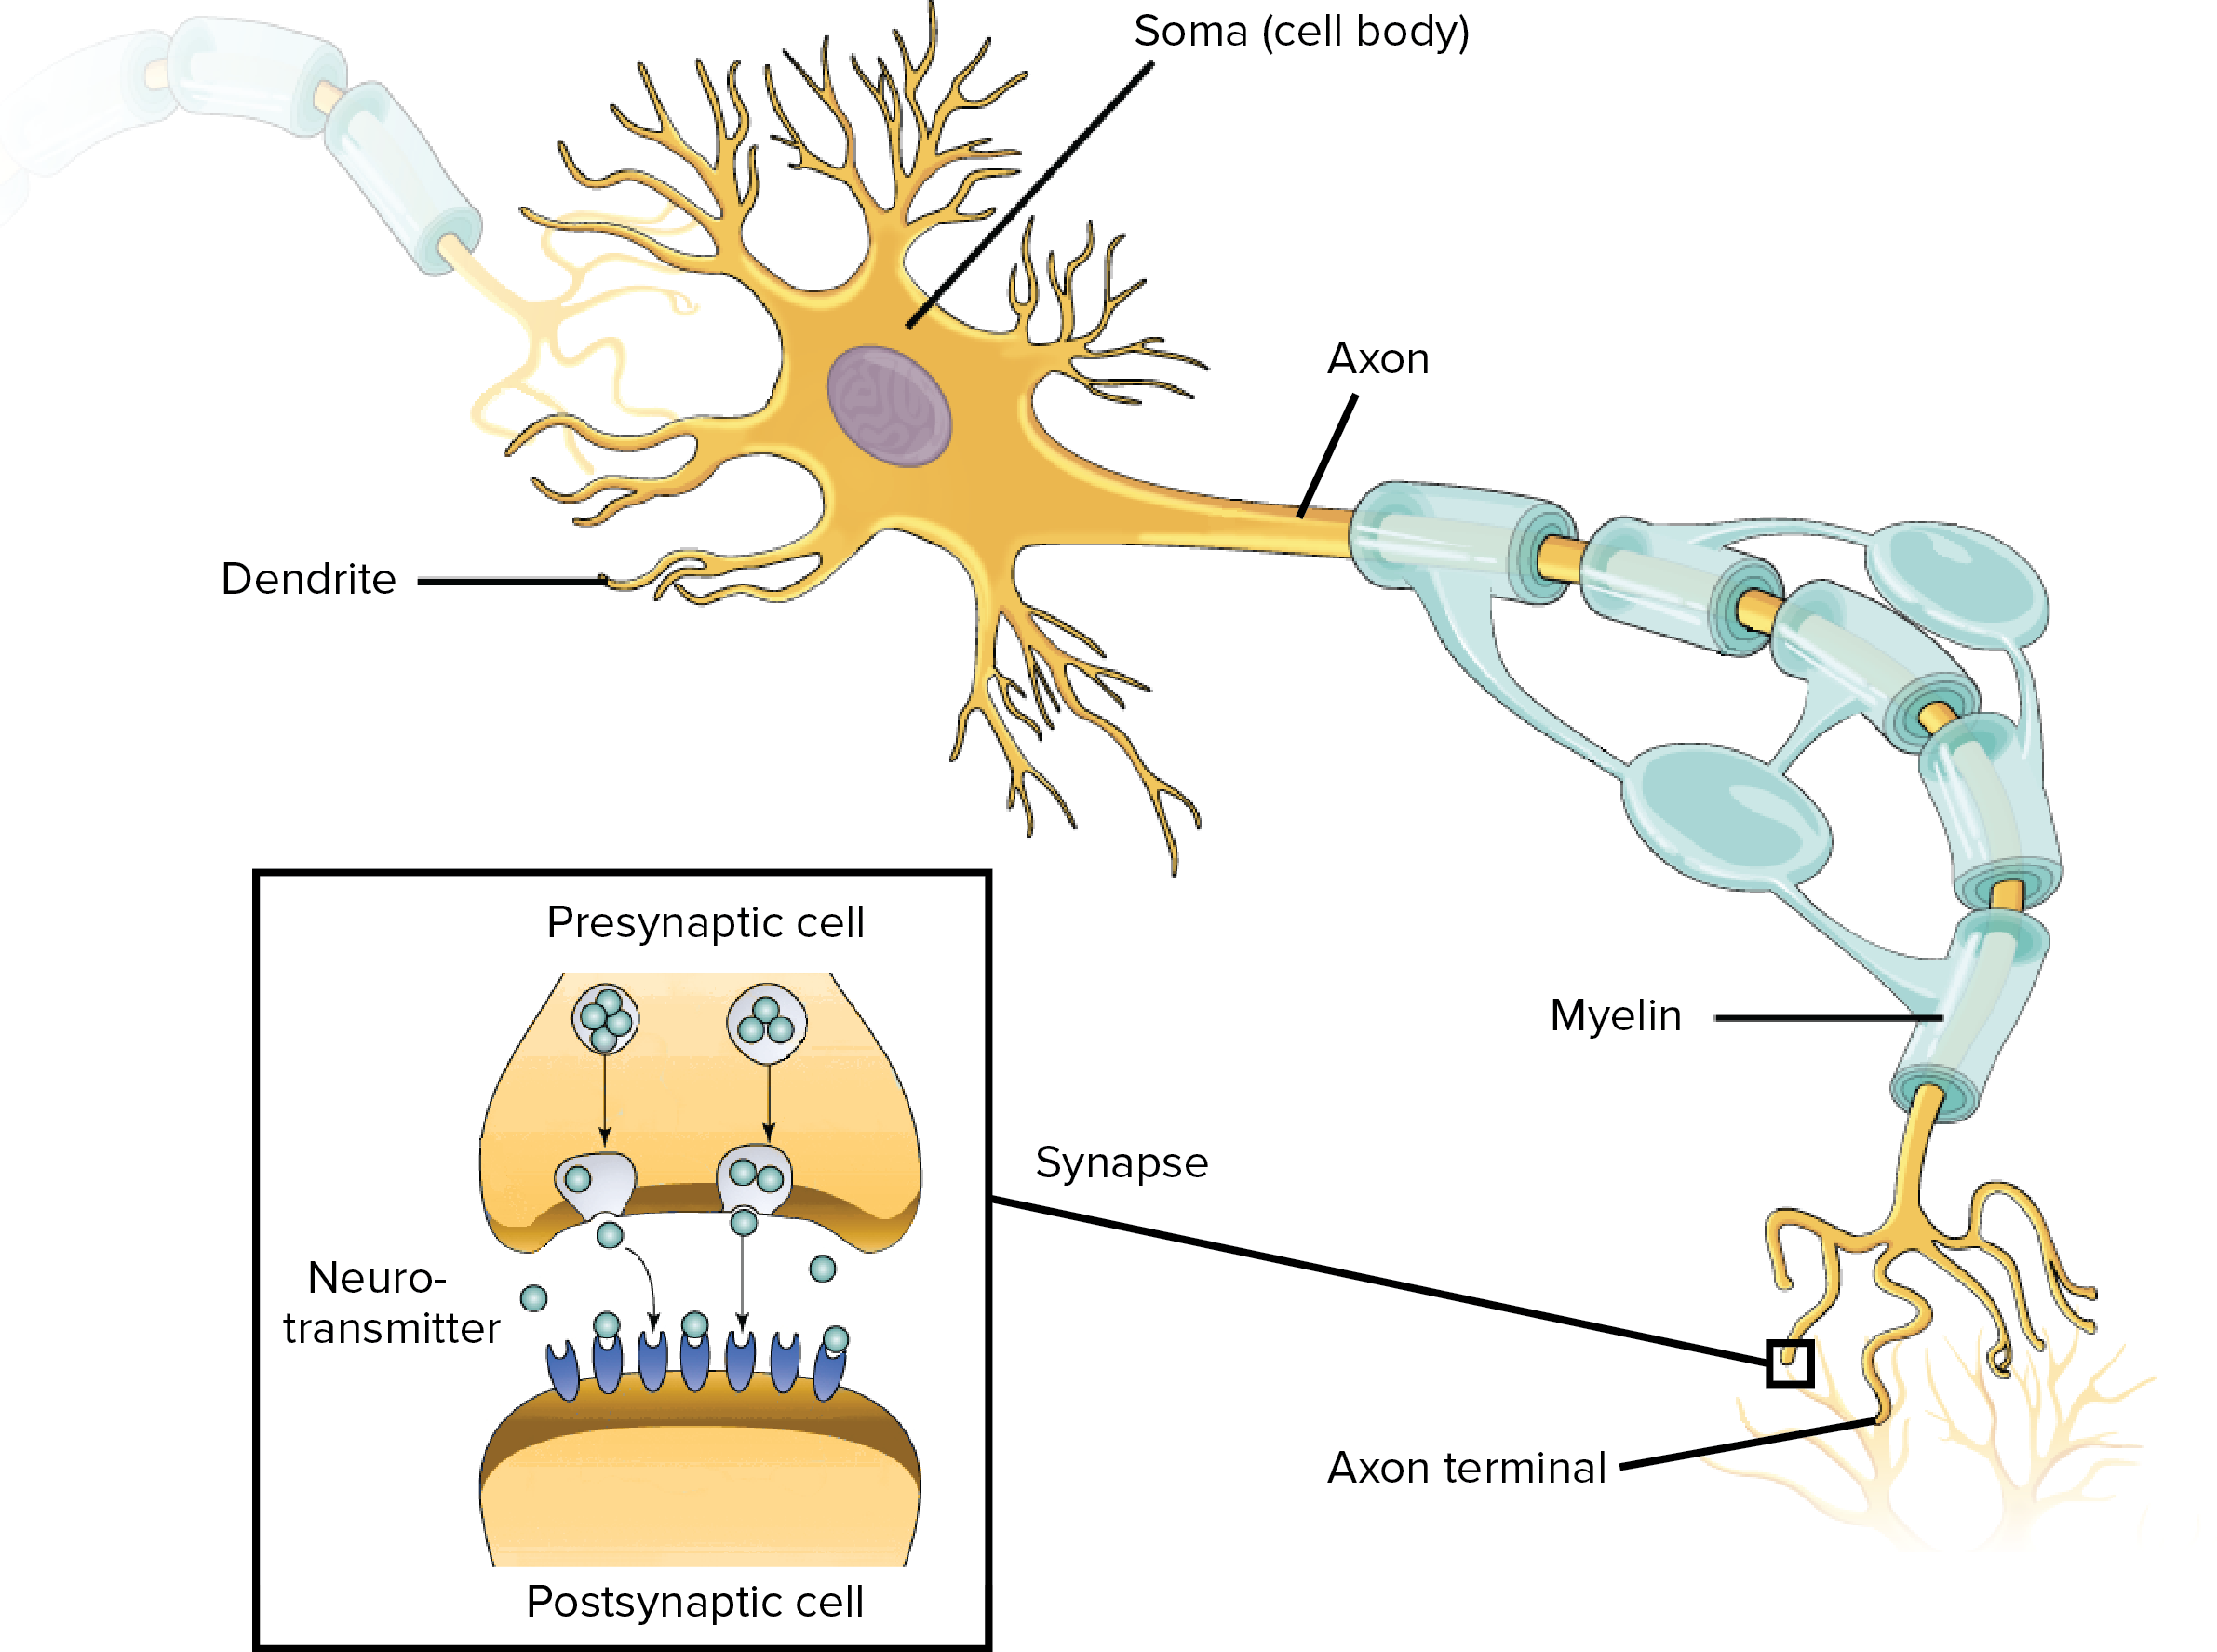
\includegraphics[width = 1\hsize]{figures/neuron.png}
\caption{Structure of a neuron with one of its synapse (image adapted from \cite{neuron}).}
\label{fig:neuron}
\end{figure}

On Fig.~\ref{fig:neuron}, there is a neuron with the \textit{Soma} being its body. \textit{Neurons} are the building blocks of the human brain and their electrical current generates \textit{action potentials}, also called voltage \textit{spikes}, when reaching an excitatory state. Each \textit{neuron}'s voltage is modulated by incoming spikes received from its \textit{dendrites}, and can send out spikes of its own through \textit{axon terminals}. All spike exchanges occur in the \textit{synapse}, where \textit{neurotransmitters} from the \textit{pre-synaptic cell} (axon terminal) will be transferred to the \textit{post-synaptic cell} (dendrite), which will update the voltage in the neuron. When this voltage hits a certain threshold, the neuron \textit{fires} a voltage \textit{spike}. Then, the \textit{spike} goes through the \textit{axon}, accelerated by the \textit{myelin} structure, and frees neurotransmitters in the outbound synapses which will in turn propagate the spike to other neurons. \\

Two main classes of models are implemented in \texttt{sPyNNaker}, describing how neurons fire in response to incoming spikes (neuron models) or describing how synapses transfer spikes based on parameters such as spike \textit{frequency} or \textit{time interval} (synapse model). The details of these models are not relevant for the needs of this Page Rank project, but we still show below a minimal example of a spiking neural network simulation. The example below (adapted from \cite{pynnsim}) uses the \texttt{IF\_curr\_exp} neuron model and the \texttt{StaticSynapse} synapse model, which are defined in PyNN \cite{pynn} but not detailed here as they are not relevant for the project. \\

\begin{minted}{python}
import spynnaker8 as sim

# Setup SpiNNaker with for 1 microsec time steps
sim.setup(timestep=1.0)

# Define a population of 1 neuron that will spike once at time t=0
pIn = sim.Population(1, sim.SpikeSourceArray(spike_times=[0]), label="input")
# Define a population of 1 neuron with neuron model `IF_curr_exp'
pOut = sim.Population(1, sim.IF_curr_exp(), label="output")
# Define a synapse link pIn -> pOut with synapse model `StaticSynapse'
sim.Projection(pIn, pOut, sim.OneToOneConnector(),
               synapse_type=sim.StaticSynapse(weight=5, delay=1))

# Set spikes and voltage to be recorded at each time step
pOut.record(["spikes", "v"])

# Starts the simulation
sim.run(10) # simulation run time in ms

# [Omitted] Collect and display recorded data...
\end{minted}

This example creates a neural graph where two populations (i.e. groups) of one neuron each are linked together by a directed arc from \texttt{pIn} to \texttt{pOut}. Using biology terms, this means we define the neuron in \texttt{pIn} to have an axon linked to a synapse with a dendrite of the neuron in \texttt{pOut}. Then, we indicate we want the simulation to record the voltage over time of the receiving neuron together with to time steps when a spike was fired. Finally, we can run the simulation for 10 milliseconds and display the recorded data as shown in Fig.~\ref{fig:simple_spynnaker8}. The full code is given in Appendix \ref{app:a}.

\vspace{-0.1cm}
\begin{figure}[hbtp]
\centering
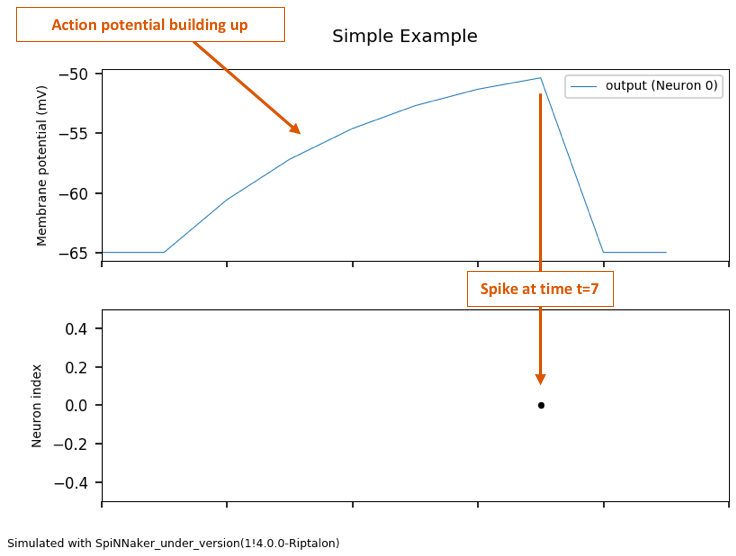
\includegraphics[width = 0.8\hsize]{figures/simple_spynnaker8.png}
\caption{Voltage and spikes fired over time \texttt{sPyNNaker8} simulation.}
\label{fig:simple_spynnaker8}
\end{figure}

This example is quite intuitive and straightforward, so we can image that even for complex simulations the implementation on sPyNNaker will not be a challenge. However, this framework is very specific and, for reasons detailed in the project section \ref{sec:impl}, Page Rank computations cannot be expressed in this framework. Consequently, we also give some background for alternative applications of SpiNNaker, those that cannot be expressed as spiking neural networks and that are still efficiently computed on SpiNNaker. \\

\subsubsection{Alternative applications} \label{sec:aa}

When the targeted application is not a spiking neural network, \textit{sPyNNaker8} is usually too constraining as it is high-level and makes design assumptions that only fit a spiking neural network.

\paragraph{Heat Equation Solver} \label{sec:hes}

To illustrate this issue, let us take the example of a heat equation solver running on SpiNNaker. Such a simulation is defined by a 2D grid where each cell iteratively propagates its heat to its neighbours according to a fixed set of rules. The algorithm propagates heat step-by-step until a convergence point is reached at time $k$, that is when the L1-norm $|| \textnormal{grid}_k - \textnormal{grid}_{k-1} ||_1 $ is less than a given threshold. Regarding the SpiNNaker implementation, a design requirement that disqualifies \texttt{sPyNNaker8} upfront is the need for each node to propagate some of its state (its heat). Indeed in the \texttt{sPyNNaker} implementation, each neuron is managed alongside its inbound synapses. When a neuron A spikes and it points to neuron B, A will send a packet to tell neuron B it spiked but without carrying any information about the intensity of the spike (40-bit packet with no payload, see \ref{sec:pf}). This is because all spikes have the same intensity (configurable in simulation parameters) and modelling a smaller spike is delegated to the synapse. Consequently, no state can leave the neuron which conflicts with the requirement for a heat node to propagate some of its local heat. \\

\begin{wrapfigure}[18]{r}{0.5\textwidth}
    \begin{center}
    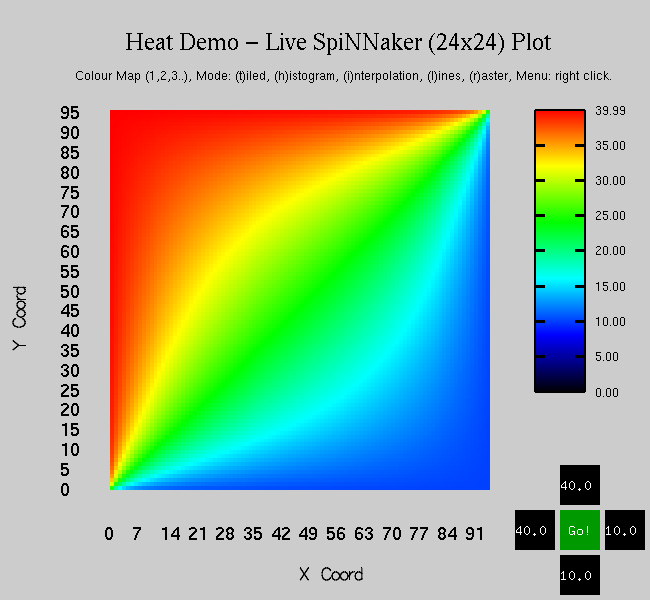
\includegraphics[width=0.48\textwidth]{figures/heatvis.png}
  	\caption{The visualiser for the Heat Equation solver (image from \cite{heatvis}).}
  	\label{fig:heatvis}    
    \end{center}
\end{wrapfigure}

As a result, the \texttt{SpiNNakerGraphFrontEnd} was chosen to implement the heat equation solver, which can be found in an earlier version of the examples shipped with the module \cite{gfeheat}. The solver also had a visualiser that was directly exchanging SCP/SDP packets with SpiNNaker to show a live view of the grid with its heat converging; see Fig.~\ref{fig:heatvis}. Part of the tooling kit built for SpiNNaker involves a few visualising tools which we do not use for this project. This particular visualiser is a custom one made solely for the purpose of this example, but it relies of the same patterns as the general-purpose ones. \\


\paragraph{Markov Chain Monte Carlo Inference (MCMC)} \label{sec:mcmc}

This last example is also very relevant for us as implementing MCMC requires the propagation of some state across the system. Like the Heat Equation Solver, the data flow moves across the network. The results of this project were published in a paper \cite{markov-on-spinn} co-authored by Steve Furber, the head of the Advanced Processor Technologies Group (APT) at the University of Manchester that designed SpiNNaker. \\

The project uses Neural Sampling and Gibbs sampling with Bayesian networks as a benchmark to test the computational abilities of SpiNNaker machines on alternative applications. Running these models is very CPU-intensive and offers parallelism opportunities, hence the choice of SpiNNaker. Implementation-wise, the \texttt{SpiNNakerGraphFrontEnd} was also used and a framework was built around it to let researchers define new Markov Chain models. \\

In addition to the design decisions made, the interesting takeaway from that project is the scaling results observed, see Fig.~\ref{fig:markov-spinn-results}:

\begin{figure}[hbtp]
\centering
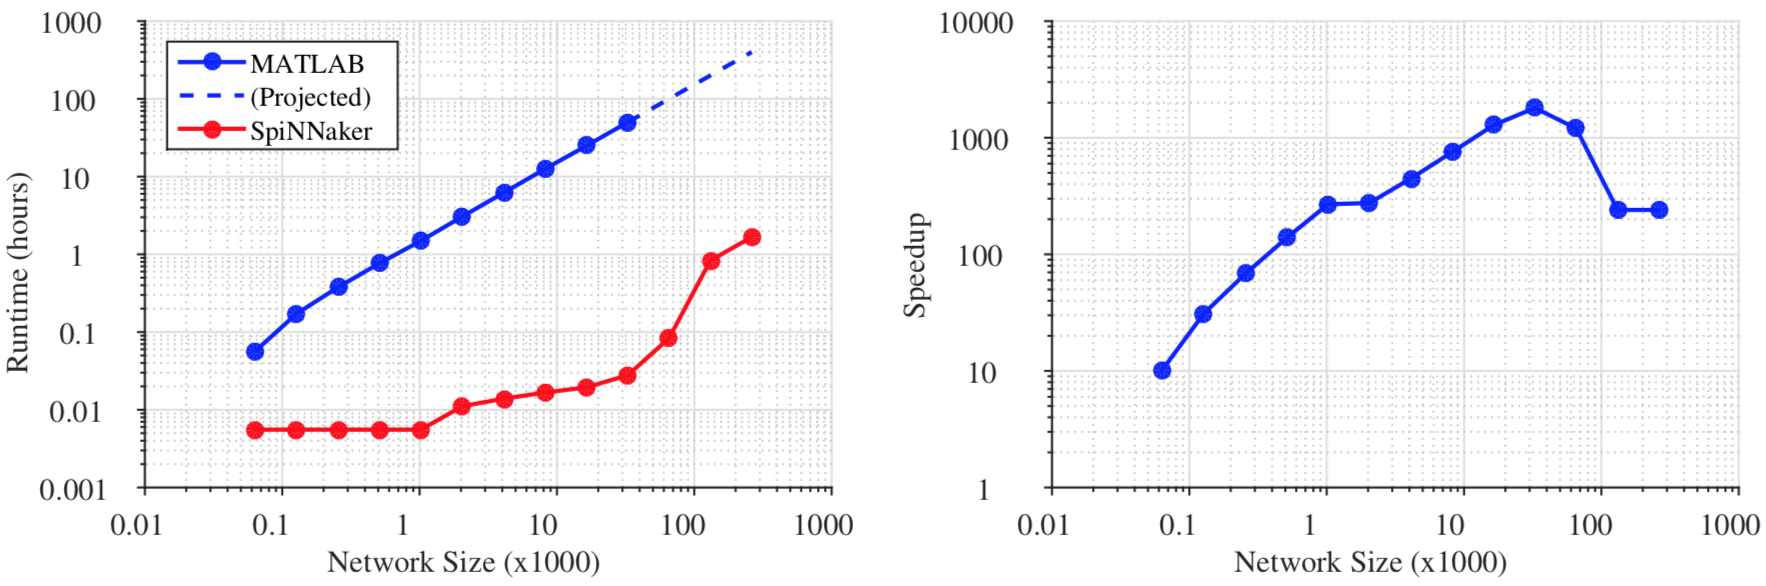
\includegraphics[width = 1\hsize]{figures/markov-spinn-results.png}
\caption{Runtime and speedup comparisons between 50,000 iterations of single-threaded Neural Sampling on a PC (Intel Core i7 3770K processor) in MATLAB and parallel Neural Sampling with spiking neurons on SpiNNaker (48 chips) (image and caption adapted from \cite{markov-on-spinn}).}
\label{fig:markov-spinn-results}
\end{figure}


First of all, we can note that it is probably inconsistent to compare the running times of two machines of such a different nature, so we will not be concluding anything from the running times alone. \\

Nonetheless, the scaling curves on each machine (a unit-less version of the runtime graph on Fig.~\ref{fig:markov-spinn-results}) are very relevant. We can observe that the simulation scales linearly on a PC whereas on SpiNNaker the scaling is sub-linear up to a network size of 100,000 nodes. [TODO: try to relate to the resources used to explain it if possible...] This trend motivated projects like this one, by demonstrating that the scaling potential on SpiNNaker was significant. It also exhibits another potential pitfall of SpiNNaker, which relies on a network to propagate messages. The drop in performance from 100,000-node graphs is due to network congestion that physically limits the scalability potential of algorithms that need to exchange too much state at once. This will be a parameter to look for in this project's implementation of Page Rank: can we anticipate a drop in performance for some given graph topologies? \\

\vspace*{-0.1cm}
Having covered all the background material needed, we can now review the successive implementations that constitute one of the contributions of this project.

